%% ****** Start of file apstemplate.tex ****** %
%% 
%%
%%   This file is part of the APS files in the REVTeX 4 distribution.
%%   Version 4.1r of REVTeX, August 2010
%%
%%
%%   Copyright (c) 2001, 2009, 2010 The American Physical Society.
%%
%%   See the REVTeX 4 README file for restrictions and more information.
%%
%
% This is a template for producing manuscripts for use with REVTEX 4.0
% Copy this file to another name and then work on that file.
% That way, you always have this original template file to use.
%
% Group addresses by affiliation; use superscriptaddress for long
% author lists, or if there are many overlapping affiliations.
% For Phys. Rev. appearance, change preprint to twocolumn.
% Choose pra, prb, prc, prd, pre, prl, prstab, prstper, or rmp for journal
%  Add 'draft' option to mark overfull boxes with black boxes
%  Add 'showpacs' option to make PACS codes appear
%  Add 'showkeys' option to make keywords appear
\documentclass[aps,pra,twocolumn,superscriptaddress,numerical,floatfix]{revtex4-1}
%\documentclass[aps,prl,preprint,superscriptaddress]{revtex4-1}
%\documentclass[aps,prl,reprint,groupedaddress]{revtex4-1}

% You should use BibTeX and apsrev.bst for references
% Choosing a journal automatically selects the correct APS
% BibTeX style file (bst file), so only uncomment the line
% below if necessary.
%\bibliographystyle{apsrev4-1}

\usepackage{graphicx}% Include figure files
\usepackage{dcolumn}% Align table columns on decimal point
\usepackage{bm}% bold math
\usepackage{amsmath}
\usepackage{amsthm}
\usepackage[T1]{fontenc}
\usepackage[latin9]{inputenc}
\setcounter{secnumdepth}{3}
\usepackage{amssymb}
\usepackage{hyperref}% add hypertext capabilities
%\usepackage[mathlines]{lineno}% Enable numbering of text and display math
%\linenumbers\relax % Commence numbering lines
\usepackage{braket}
\usepackage{placeins}

\usepackage{amsthm}
\newtheorem{theorem}{Theorem}
\newtheorem{corollary}{Corollary}

\newtheorem{thm}{Theorem}

\graphicspath {{Figures/}}% specifying where to look for all figures

\begin{document}

% Use the \preprint command to place your local institutional report
% number in the upper righthand corner of the title page in preprint mode.
% Multiple \preprint commands are allowed.
% Use the 'preprintnumbers' class option to override journal defaults
% to display numbers if necessary
%\preprint{}

%Title of paper
\title{Error Correction Through Error Averaging}

% repeat the \author .. \affiliation  etc. as needed
% \email, \thanks, \homepage, \altaffiliation all apply to the current
% author. Explanatory text should go in the []'s, actual e-mail
% address or url should go in the {}'s for \email and \homepage.
% Please use the appropriate macro foreach each type of information

\newcommand{\affone}{Centre for Quantum Computation and Communication Technology (CQC2T), The School of Mathematics and Physics, The University of Queensland, Australia.}
\newcommand{\afftwo}{Centre for Quantum Computing \& Intelligent Systems (QCIS), University of Technology Sydney, Australia.}
% \affiliation command applies to all authors since the last
% \affiliation command. The \affiliation command should follow the
% other information
% \affiliation can be followed by \email, \homepage, \thanks as well.
\author{Ryan J. Marshman}
%\email[]{Your e-mail address}
%\homepage[]{Your web page}
%\thanks{}
%\altaffiliation{}
\affiliation{\affone}

\author{Austin P. Lund}
\affiliation{\affone}

\author{Peter P. Rohde}
\affiliation{\afftwo}

\author{Timothy C. Ralph}
\affiliation{\affone}

%Collaboration name if desired (requires use of superscriptaddress
%option in \documentclass). \noaffiliation is required (may also be
%used with the \author command).
%\collaboration can be followed by \email, \homepage, \thanks as well.
%\collaboration{}
%\noaffiliation

\date{\today}

\begin{abstract}
Given the current drive to witness the supremacy of quantum computing it is imperative to design implementable error correction protocols. In this paper we propose and investigate Error Averaging, a novel method of error detection and reduction. Error averaging improves on existing methods of error detection and correction by not relying on ancillary photons or complicated control and correction circuits \cite{Perfect}. Error averaging can be applied to any quantum computing architectures which satisfies two requirements, both of which are satisfied automatically by Linear Optical Quantum Computing (LOQC). Error averaging will be introduced first in a general context followed by a series of proof of principle examples. Two methods of Error Averaging are then compared to determine the most effective manner of implementation and probe the related error thresholds. It is hoped that by employing existing methods of protecting against losses that this system could be used as a method of error correction in its own right.
\end{abstract}

% insert suggested PACS numbers in braces on next line
\pacs{}
% insert suggested keywords - APS authors don't need to do this
%\keywords{}

%\maketitle must follow title, authors, abstract, \pacs, and \keywords
\maketitle

% body of paper here - Use proper section commands
% References should be done using the \cite, \ref, and \label commands
\section{Introduction \label{intro}}
Quantum technology and in particular Quantum computing is a very promising area of research with the potential to lead to some of the most significant technological advances in recent times. There are, however, still many hurdles before universal quantum computing is achieved. The focus of this paper will be on the hurdle of error correction. The Error Averaging protocol requires the input qubits to be placed in a spatial superposition and restricts the effect that any applied unitary has on the vacuum. Both of these requirements are satified by LOQC and as such this will form the basis for most of this paper.

Error Averaging in its current state forms a rudimentary form of error correction which currently acts to distil errors form the system in such a way that they can be post selected away. Figure \ref{fig:output_probabilities} shows how Error Averaging by itself lowers the probability of success, but increases the probability of obtaining the correct result after post selecting on no errors being detected. The variance of the errors in the system have been shown to scale as $\frac{1}{N}$ where $N$ represents the amount of correction or equivalently the number of copies of the system.

\begin{figure}
	\begin{centering}
		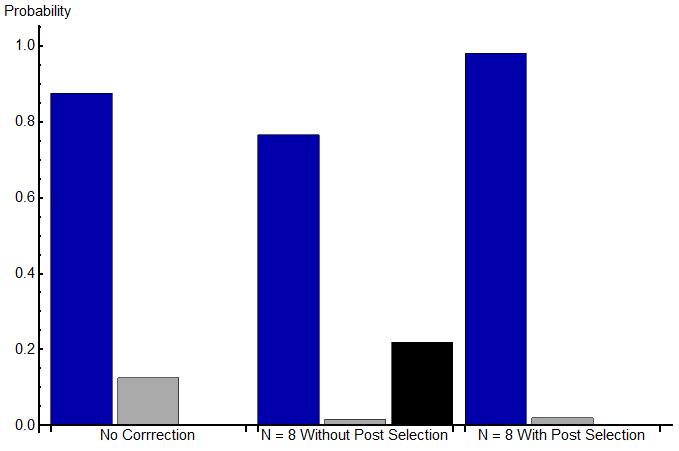
\includegraphics[width=\columnwidth]{prob_distributions.png}
	\end{centering}
	\caption[Comparison of output probability distributions with and without Error Averaging.]{Comparison of output probability distributions with and without error 	averaging. This also demonstrates the effect post selection has on the output distribution. The blue bars represent the probability of observing the photon in the correct output mode, grey corresponds to observing the photon in the incorrect output mode and black corresponds to observing the photon in any of the error detection modes. The probabilities are based on a single photon in a Mach-Zehnder interferometer with an individual phase shifters variance $v=0.5\ \textrm{rad}^{2}$. This high variance is chosen.} 
	\label{fig:output_probabilities}
\end{figure}

The next section introduces the details and results for a general set-up. This is done to both explain how Error Averaging is implemented and demonstrate its effect on an output state. Section \ref{implementation} includes numerous proof of principle examples which serve to highlight the effects of Error Averaging with a focus on the scaling for the probability of success. LOQC will serve as the architecture for all these examples. The feasibility of Error Averaging will be considered including a detailed discussion of some of the underlying assumptions made in the examples below can be found in section \ref{Feasibility section} followed by some concluding remarks.

% NOTATION SUGGESTION: Use \hat{} for Fock space operators and no hat for normal matricies.
\section{General Unitary Averaging\label{gen case}}

Here we are concerned with the case of bosonic linear scattering networks.  These are evolutions of a multi-mode bosonic field where the Heisenberg equations of motion for the anhillation operators of each mode can be written as a linear combination of all anhillation operators.  That is, if $\mathcal{U}_U$ is a unitary operation on a $m$ mode system, then
\begin{equation}
	\mathcal{U}_U a_i \mathcal{U}_U^\dagger = \sum_j U_{ij} a_j
\end{equation}
where, to preserve commutation relationships, $U$ must be a unitary matrix.  It is the network matrix $U$ that we will focus on.

Consider a linear network whose elements are those of a Discrete Fourier Transform (DFT).  That is, we have an Hisenberg style evolution between mode annihilation operators of the form
\begin{equation}
	a_{j,r} \rightarrow \frac{1}{\sqrt{N}} \sum_{k=0}^{N-1} \omega^{rk} a_{j,k}	
\end{equation}
where $\omega = e^{-i2\pi /N}$ and zero-indexing of the modes has been used to simplify this expression.  The first subscript for the annihilation operator denotes the input mode and the second describes a quantity of redundancy $N$ which we explain shortly. 

We then act the $N$ copies of a target unitary $U$.  By this we mean that there is some variation between the copies but the intention was to implement the unitary $U$.  This can be described by the transformation
\begin{equation}
	a_{j,r} \rightarrow \sum_{l=0}^{m-1} (U_r)_{lj} a_{l,r}.
\end{equation}
where $N$ noisy copies of $U$ are made, denoted here as $U_1, U_2, \ldots, U_N$. 

After this the DFT matrix is applied again.  This results in the overall transformation
\begin{equation}
	a_{j,r} \rightarrow \frac{1}{N} 
	\sum_{l=0}^{m-1} \sum_{k,k^\prime=0}^{N-1}
	(U_{k^\prime})_{lj} \omega^{(r+k)k^\prime} a_{l,k}.
\end{equation}
We consider the case where all redundant modes are initialised in the vacuum state and post-select on the cases where no photons are present in the output of the redundant modes.  This means that we only need consider the parts of this transformation expression where the second subscript of the annihilation operator is zero.  In this case we have
\begin{equation}
	\label{sum_transformation}
	a_{j,0} \rightarrow \frac{1}{N}\sum_{l=0}^{m-1} \sum_{k^\prime=0}^{N-1}
	(U_{k^\prime})_{lj} a_{l,0} = \sum_{l=0}^{m-1} (M_N)_{lj} a_{l,0}
\end{equation}
where $M_N$ is a matrix defined by
\begin{equation}
	M_N = \frac{1}{N} \sum_k U_k.
\end{equation}
This matrix is then the effective linear network matrix for the post-selected system.  It includes information about the probability of success and so in general it will be not unitary.  The remainder of this paper is directed towards analysing the scenaiors that arise from the multitude of choices for $U_k$ that form expression.

For the main theorem of our work we consider a general linear network described by a unitary network matrix $U$ with any dimensionality. 

%Theorem~\ref{Theorem 1} below states that given access to $N$ linear networks $\{U_1,U_2,\ldots,U_N\}$ which are randomly distributed such that for all $i \in {1,\ldots,N}$, and given $U_{r,s}=\alpha_{r,s}e^{i\theta_{r,s}}$, $\langle \left(\theta_{i}\right)_{r,s} \rangle = \theta_{r,s}$, $\left|\left(\alpha_{i}\right)_{r,s}-\alpha_{r,s}\right|\ll1$ and $Var(U_i) = \sigma_i^2 < \infty$  the mean values of these unitaries approaches $c\times\hat{U}$, where $0\le c\le1$, in the same sense as the central limit theorem. By the central limit theorem we also see that the variance, $\sigma_{i}^{2}$, scales as $\frac{1}{N}$.

\begin{theorem}
\label{Theorem 1}
Given $N$ linear networks described by unitary matricies $\{U_1,U_2,\ldots,U_N\}$ that are random with independent and identically distributed statistics such that for all $i~\in~{1,\ldots,N}$, $\langle U_i \rangle = M$.  Then the random variable 
\begin{equation}
	\label{sum_unitary}
	M_{N}=\frac{1}{N}\sum_{i=1}^{N}U_{i}
\end{equation}
is a matrix with mean value $M$ and whose matrix elements have variance scaling as $O(1/N)$.
\end{theorem}

\begin{proof}\label{Proof 1}
Our aim in the proof is to use the central limit theorem.  Consider matrix element $r,s$ of $M_N$.  This is a random variable
\begin{equation}
	\left(M_N\right)_{rs} = \frac{1}{N} \sum_{i=1}^N \left(U_i\right)_{rs}.
\end{equation}
As the matrix elements $(U_i)_{rs}$ are constructed from unitary matrices, their magnitude is bounded by $1$.  Given this finite domain, the real and imaginary parts have maximum variance and covariance of $1$ (though these extremal values are not simultaneously achievable).  Given this bounded variance, we can use the central limit theorem to conclude that the matrix element $\left(M_N\right)_{rs}$ is a random variable with mean value $M_{rs}$.
The variance of the real or imaginary part of $(M_N)_{rs}$ is then upper bounded by $1/N$ as per the central limit theorem.
\end{proof}

The question now is what forms can the mean average matrix $M$ can take.   First we consider the trivial case where the unitary matrices are $1 \times 1$ dimensional.

\begin{corollary}
\label{Corollary 1}
	If each $\{U_1,\ldots,U_N\}$ are $1 \times 1$-dimensional, then $M$ is a complex number with magnitude $|M| \leq 1$.
\end{corollary}
\begin{proof}
	Write $U_k = e^{i \theta_k}$ where $p(\theta)$ is the probability density function for each of the angles $\theta_k$. From Theorem~\ref{Theorem 1} we need to compute the mean value 
	\begin{equation}
		M = \int^\pi_{-\pi} e^{i\theta} p(\theta) \mathrm{d}\theta. \label{eq:single parameter, single mode}
	\end{equation}
This is exactly the characteristic function of $p(\theta)$ evaluated at $1$.  The characteristic function is complex valued and has bounded magnitude of $1$, which is the desired result.
\end{proof}

By corollary~\ref{Corollary 1} it can be concluded that for the $1\times1$-dimensional case we can write $M=cU$ where $0 \leq c \leq 1$ and $U=e^{i\theta}$ has magnitude 1.  

% NOTE TO SELF(APL): Talk more about post-selection and M in this section
%Here we can identify the coefficient $c$ as the probability of success and as such, after post selection, the matrix $c\times U_{N}$ can be renormalised to a unitary matrix $U_{N}$ with $\lim_{N\rightarrow\infty}U_{N}=U$. 

Next consider higher dimensional matrices whose distribution is generated by a single parameter.  In this case, for any hermitian matrix $T$, which is can be thought of as an infinitesimal generator from the $u(n)$ Lie algebra, we have
\begin{equation}
	M=\int e^{i\theta T}p(\theta)d\theta 
	\label{eq:single parameter, multi-mode}.
\end{equation}
We can make a change of variables in $\theta$ so that the distribution is changed to one that has mean zero
\begin{align}
	M&=\int e^{i(\mu + \theta^\prime)T} p(\mu + \theta^\prime) d\theta^\prime\\
	&= e^{i\mu T} \int e^{i\theta^\prime T} \bar{p}(\theta^\prime) d\theta^\prime
\end{align}
where $\bar{p}(\theta) = p(\mu + \theta)$ so that it has mean value zero.  By expanding the matrix exponential this expression can be written as
\begin{equation}
	M=\sum_n \frac{(iT)^n}{n!} \int \theta^n p(\theta) d\theta,
\end{equation}
which now relates to the moments of the underlying distribution in $\theta$. If $p(\theta)$ were a Gaussian distribution with mean zero and variance $\sigma^2$ then we can write
\begin{equation}
	M = \sum_{n \in even} \frac{(iT)^n}{n!} (n-1)!! \sigma^n
\end{equation}
where $n!! = n(n-2)(n-4)\dots$ is the double factorial.  This series can be written back in the form of a matrix exponential, and by reindroducing the mean value we have
\begin{equation}
	M = e^{i\mu T} e^{-\frac{\sigma^2}{2} T^2}
\end{equation}
If $T^2=I$, which would be the case when choosing a Pauli matrix for $T$, then this expression would simplify to
\begin{equation}
M=Ue^{-\frac{\sigma^2}{2}}  \label{eq:Gaussian Psuccess}
\end{equation}
where $U$ is the unitary generated by the average parameter for $p(\theta)$.  The decaying exponential for the magnitude depends only on the variation in the distribution of $\theta$.

In the full parameter case, provided the target unitary $U$ again commutes with all errors a similar result can be found as discussed in corollary \ref{Corollary 2}.

\begin{corollary}
\label{Corollary 2}
If $\{U_1,\ldots,U_N\}$ are random $n$-dimensional unitaries such that $U_k = U exp\{i \sum_l \alpha_{kl} T_l\}$ with $n^2$ generators $T_l$ that are all hermitian and satisfy $T_l^2=I$, the parameters $\alpha_{kl}$ distributed independently with PDF $p_{l}(\alpha_l)$ which are all Gaussian with mean zero and small (but possibly different) variances so that they all $U_k$ approximately commute with each other, then $M = c U$ where $0 < c < 1$ and $U$ is a unitary matrix.
\end{corollary}
\begin{proof}
We will extend the proof of Corollary~\ref{Corollary 1} to the $n$-dimensional case.  From the independance of the distributed parameters, we can write a PDF for all parameters as $p(\alpha_1,\ldots,\alpha_{n^{2}}) = p_1(\alpha_1)\times\ldots\times p_{n^2}(\alpha_{n^{2}})$.  
%For any Write where $T_l$ are generators of the $u(n)$ Lie-algebra of which there are $n^2$ and $U$ is chosen so that the distribution is defined by probability density function $p(\alpha_1,\ldots,\alpha_{n^{2}})$ has mean zero. $T_l$ are chosen so that and $-\pi < \alpha_l < \pi$. 
%As all errors are taken to be independent we can also write  
The approximate mutual commutivity for this expansion means 
\begin{widetext}
\newcommand{\theint}{\int^\pi_{-\pi} \ldots \int^\pi_{-\pi} \int^\pi_{-\pi}}
\newcommand{\theintd}{\mathrm{d}\alpha_1 \mathrm{d}\alpha_2 \ldots \mathrm{d}\alpha_{n^{2}}}
\begin{equation}
	\int^\pi_{-\pi} \int^\pi_{-\pi}
	[\alpha_{kl}T_{l},\alpha_{km}T_{m}] p_l(\alpha_l)p_m(\alpha_m) \mathrm{d}\alpha_l \mathrm{d}\alpha_m \approx 0 \quad \forall l,m,
\end{equation}
or in other words, that the $\alpha_{kl}T_l$ are all small with high probability.  With this we can write $M$ as
\begin{align}
	M &= U \theint
	exp\{i \sum_l \alpha_{l} T_l\} p_1(\alpha_1)\ldots p_{n^2}(\alpha_{n^{2}})
	\theintd
	\label{eq:general integral form} \\
	&\approx U \theint
	\prod_{l}exp\{i \alpha_{l} T_l\}p_1(\alpha_1)\ldots p_{n^2}(\alpha_{n^{2}})
	\theintd  \\
	&= U\int^\pi_{-\pi} exp\{i \alpha_{1} T_1\}p_1(\alpha_1) \mathrm{d}\alpha_1 	\int^\pi_{-\pi} exp\{i \alpha_{2} T_2\}p_2(\alpha_2) \mathrm{d}\alpha_2 \ldots \int^\pi_{-\pi}
	exp\{i \alpha_{n^2} T_{n^2}\}p_{n^2}(\alpha_{n^2}) \mathrm{d}\alpha_{n^2} \\
	&\approx U \prod_l e^{-\frac{\sigma_l^2 T_l^2}{2}},\label{eq:approx commuting, general case}
\end{align}
\end{widetext}
where $\sigma_l^2$ is the variance of $p_l$ and the final approximation is assuming the distribution is small so that the bounds of the integration do not matter.  Using the $T_l^2=I$ requirement on the generators the final product of exponentials can be identified with the value $c$, we have the desired result.
\end{proof}
The requirement of $T_L^2=I$ merely reflects a simplification where the generators are built from the Pauli matricies which is the constructions we will focus on in this paper.  If this is not the case then it is possible to identify the hermitian operator $\prod_l e^{-\frac{\sigma_l^2 T_l^2}{2}}$ as a state dependant decay in the amplitude of the operator.

%It should be noted that if the distribution of parameters is Gaussian but not indepenent, then there is gaurenteed to be a linear combination of parameters for which this distribution is indepdenant.  Hence by changing the generators in the apropraite way, one can always arrange this situation for Gaussian distributions of the parameters $\alpha_{kl}$.


%From Corollary \ref{Corollary 2} and given our previous result for a Gaussian error distribution we can conclude that
%\begin{equation}
%M = U\prod_{l}^{n^2}e^{-\frac{\sigma_{l}^{2}}{2}}\label{eq:approx commuting, general case}
%\end{equation}
%To be clear this results requires that the errors are small such that they approximately commute with one another and with the target matrix $U$. The distributions $p(\alpha_{l})$ are also, in general, not equivalent, even if each component within a system has an equivalent error distribution the beam splitter parameters will not necessarily corresponds directly to the coefficients of the generators in the Lie algebra. 

Finding explicity closed forms for the matrix $M$ outside of the situations just outlined is an open problem.  In the most general case, $M$ is not be proportional to a unitary matrix.  Furthermore, is not gaurenteed that $M$ satisfy the conditions for a normal matrix and hence cannot be unitarily diagonalised.  So it is unclear if this post-selected regime has any connection to unitary quantum evolution at all.  Nevertheless, we will begin to examine situations which approach this domain through decompositions into single parameter problems and using numerical computations.

\section{Implementation\label{implementation}}

This section demonstrates how Error Averaging can be implemented for various example systems. These examples also serve as a verification of the range of validity of approximately commuting errors assumption. It can also be noted that Equation~(\ref{sum_unitary}) can become the appropriate transformation for duality quantum computing by allowing the $U_{i}$ to be arbitrary\cite{dualityQC}.

Constructions using the DFT implementation from the previous section may be inconvenient depending on the nature of the system used.  The transformation of Eq.~(\ref{sum_transformation}) can also be achieved using an array of beam-splitters as shown in Fig.~\ref{fig:gen system}.  This beam-splitter array also has the desirable property of a nested pattern.  As shown by the bounding rectangles in Fig.~\ref{fig:gen system}, the outer and inner layers share the same basic structure. 
%
\begin{figure}[tbh]
	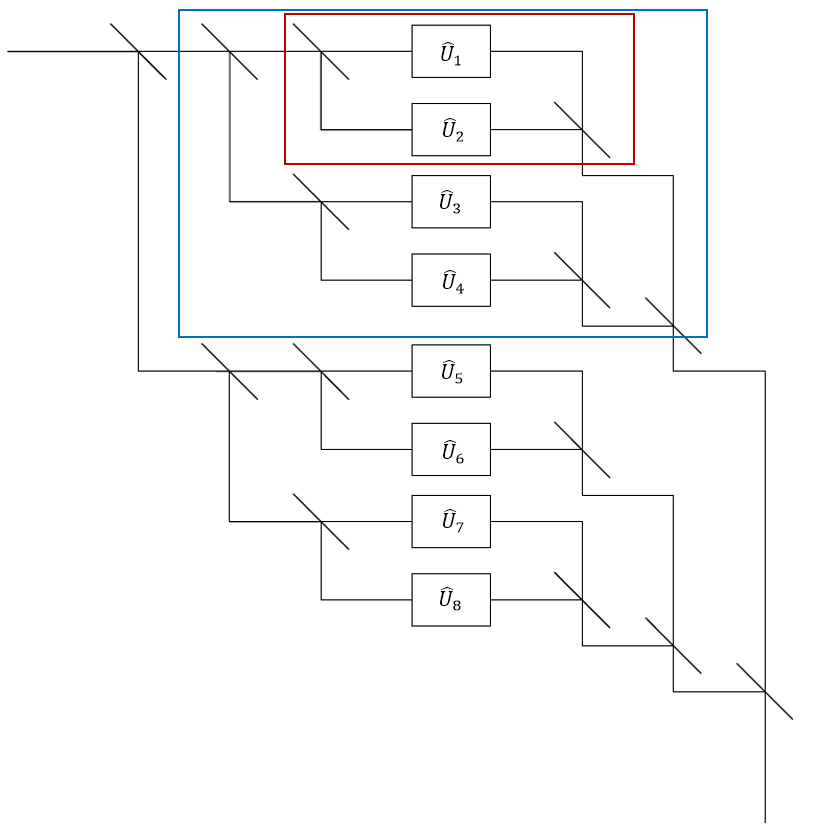
\includegraphics[width=\columnwidth]{unitaries.PNG}
	\caption{\label{fig:gen system}Diagram showing the innermost components marked with $\hat{U}_i$ being error averaged eight times using fourteen beam splitters. Note that for clarity the error detection modes are not included. See figure \ref{fig:MZ_setup} for an example explicitly including the error detection modes. The inner fixed beam splitters can be considered error averaged four times by taking the component of the system in the red box as a smaller system which is error averaged. Similarly the system in blue box which is effectively being averaged twice.}
\end{figure}
	
%The following section discusses the results of numerical simulations for various systems implementing Error Averaging. To understand why linear optics was the chosen implementation consider the two key requirements of implementation. The first requirement is that the fundamental particle used as the computational qubit can be placed in a spacial superposition. The second requirement is that any employed unitary $\hat{U}$  does not act on the vacuum, that is $\hat{U}\left|0\right>=\left|0\right>$. Although these seem restrictive, LOQC automatically satisfies both of these requirements. A spacial superposition can be created easily using beam splitters and any linear optical unitary cannot, by definition, affect the vacuum.
	
%	Within the LOQC architecture, the following discussion will be agnostic about the specific encoding method by working in the Fock basis. In this way both single and dual rail encoding can be corrected and as such will generally not be considered in all further discussions.

Initially we will focus on phase errors as this case is well understood and sets the stage for developing more complex scenarios.  The fundamental components in linear networks are phase shifters and beam splitters.  All networks can be generated by arranging networks of these elements~\cite{reck}.  Carolan et. al.~\cite{ULO} have experimentally probed a linear network where all possible networks can be generated using controllable phase shifters with fixed beam splitters. The basic idea is to replace each beam splitter in a network decomposition with a Mach Zehnder (MZ) interferometer consisting of a controllable phase shifter in one arm and two fixed $50:50$ beam splitters. In their experimental implementation they demonstrated the ability to implement many quantum logic gates and linear optical protocols with a high fidelity.  Using this experiment as a guiding framework we considered phase errors as a dominate error source as they were the parts of the network subject to variation. 
	
Following this framework we assume $50:50$ beam splitters which are ideal and the phase shifts are the source of all errors. The applied phase shift can then be written as $e^{i(\theta+\delta)}$ where, for the identity, $\theta=0$ and $\delta$ is a random variable represing the errors.  In terms of the constructions used in Section~\ref{gen case}, this corresponds to Equation \ref{eq:single parameter, multi-mode} with $T=\begin{bmatrix}	0 & 1 \\	1 & 0 \\\end{bmatrix}$ and $M=e^{i\delta T}$ where we have set $U=\mathbb{I}$. This distribution for $\delta$ is taken to be Gaussian with mean $0$ and variance $v$. 

%Need to come back to this.  Not sure what it means.
We will initially consider a single beam splitter for a one and two photon inputs with $N$ internal phase shifters where $N=2^{n},n\in\mathbb{N}$. As the entire system is implementing a beam splitter it has two desired input and output modes. However as $N$ increases so too does the actual number of input and output modes. All of these extra input modes are effectively ignored by being set to the vacuum state $\left|0\right\rangle $. The extra output ports all have photo-detectors which will be post selected on being zero.
		
	
\subsection{1 photon N arbitrary \label{1 photon N arbitrary}}
	
Here we will consider single photon inputs into arbitrarily sized redundant encodings (counted by $N$).  As a measure of performance, we will use the redundant encoded circuit on one arm of a Mach-Zender (MZ) interferometer.  This system is shown in Figure \ref{fig:MZ_setup} for the $N=2$ case.  In an ideal interferometer an input single photon state will be transferred to a single output with a probability that varies sinusoidally between 100\% and 0\%.  Deviations from this are attributed to non-ideal interferometer performance. 
\begin{figure}[tbh]
	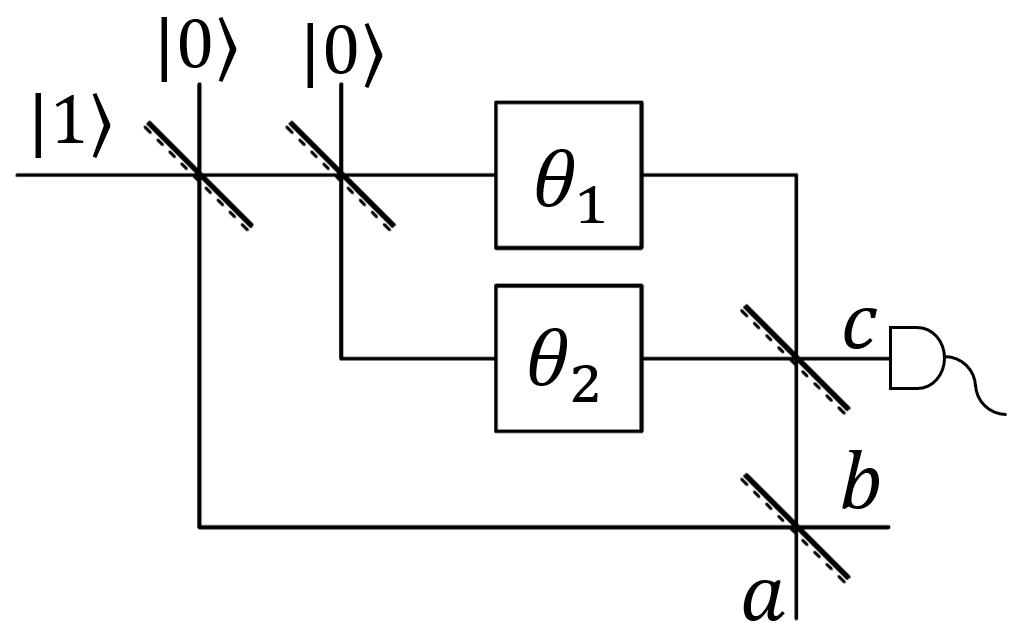
\includegraphics[width=\columnwidth]{2N1P.png}
	\caption{\label{fig:MZ_setup}Diagram of Mach-Zender interferometer with a redundantly encoded phase shift of $N=2$, that is, two phase shifts. $a$ and $b$ label output modes and $c$ labels an error detection mode. The input state shown is the one used for all single photon calculations and more vacuum modes are introduced for larger $N$. The phase shift elements are marked with $\theta_{i}$ and are the only source of error for the applied phase shift.}
\end{figure}
	
A single photon input state can be written an $\left|\phi\right\rangle = \hat{a}^{\dagger}\left|0\right\rangle $.  This state is the input for the MZ interferometer.  The redundant encoding in one arm is performed using 50:50 beam-splitters and the objective is to apply some phase shift of angle $\theta$.  The resulting output state is
\begin{widetext}
\begin{equation}
	\ket{\psi} = \left(
	\left( \frac{e^{i\theta}}{2} \left\{\frac{1}{N}\sum_{j=1}^{N}e^{i\delta_{j}}\right\} + \frac{1}{2}\right) \hat{a}^{\dagger} 
	+ \left(\frac{e^{i\theta}}{2} \left\{\frac{1}{N}\sum_{j=1}^{N}e^{i\delta_{j}}\right\} - \frac{1}{2}\right) \hat{b}^{\dagger} 
	\right)
	\ket{0}.
	\label{eq:1ParbN}
\end{equation}
\end{widetext}
where $\theta_{i}=\theta+\delta_{j}$ with $\theta$ a constant and $\delta_j$ a random variable.  This output includes post-selection so terms that contain creation operators in modes that are post-selected to be vacuum are truncated. 

\emph{(NOTE: We know what this sum averages to so can we just do these calculations exactly?)}
Furthermore  in the following two sections second order Taylor approximations we used to simplify the result. 

As this linear network conserves photon number we know that for this single photon case that the output state always contains one and only one photon.  The probability that the photon is measured in a particular mode can therefore be equated to the average photon number in that mode.  Using this we can calculate the probability of observing the photon in the $\hat{a}$ and $\hat{b}$ modes without post-selection to be 
\begin{eqnarray}
	\bra{\psi} \hat{a}^{\dagger}\hat{a} \ket{\psi} & \approx & \cos^{2}\left(\theta/2\right)+\frac{v}{4N}-\frac{v\cos^{2}(\theta/2)}{2}
\end{eqnarray}
and
\begin{eqnarray}
	\left\langle \psi\right|\hat{b}^{\dagger}\hat{b}\left|\psi\right\rangle & \approx & \sin^{2}\left(\theta/2\right)+\frac{v}{4N}-\frac{v\sin^{2}(\theta/2)}{2}.
\end{eqnarray}
The redundant encoding is applied successfully when the photon exits the encoding back into the arm of the MZ interferometer.  This means the probability of success is the sum of the probabilities of the $\hat{a}$ mode and $\hat{b}$ mode.  This is 
\begin{eqnarray}
	P(\textrm{success}) & = & \bra{\psi}\hat{a}^{\dagger}\hat{a}\ket{\psi} +\bra{\psi}\hat{b}^{\dagger}\hat{b}\ket{\psi} \\
	& \approx & 1+\frac{v}{2N}-\frac{v}{2}. \label{eq:1pNarbitrary successs}
\end{eqnarray}
In the large $N$ limit, this corresponds to the linear approximation of Equation \ref{eq:Gaussian Psuccess} where we can identify $P(\textrm{success})=c$. 

To further illustrate the this error averaging when combined with post-selection, consider the case when $\theta=0$, the probability of observing the output in the correct mode without post-selection is
\begin{equation}
	\left\langle \psi\right|\hat{a}^{\dagger}\hat{a}\left|\psi\right\rangle \approx 1 - \frac{(2N-1)v}{4N}. \label{eq:1pNoPost}
\end{equation}
After post-selection this becomes
\begin{equation}
	\left\langle \psi\right|\hat{a}^{\dagger}\hat{a}\left|\psi\right\rangle \approx 1 - \frac{v}{4N}. \label{eq:1pWithPost}
\end{equation}
\emph{(NOTE: This has to be wrong as the left hand sides of both equations are the same.  I think the second equation should be divided out by something, perhaps Eq. (26))}
		
Figure~\ref{fig:post vs no post} shows how these two quantities scale with $N$. In particular, it can be seen that with post-selection the likelihood of the photon exiting the interferometer in the correct mode can be made arbitrarily close to unity by increasing $N$. Also it is seen that while the probability of success decreases for increasing $N$ this asymptotes to some fixed value. This implies that as $N$ increases, even thought the total quantity of errors added to the system increases, the effects of the combined errors on the interferometer is less. This can be understood by the process of redundantly splitting and recombining the state, tends drive noise into the error ports by interference.  This results in the state at the output modes utilised by the interferometer approaching an ideal noiseless state.
\begin{figure}[tbh]
	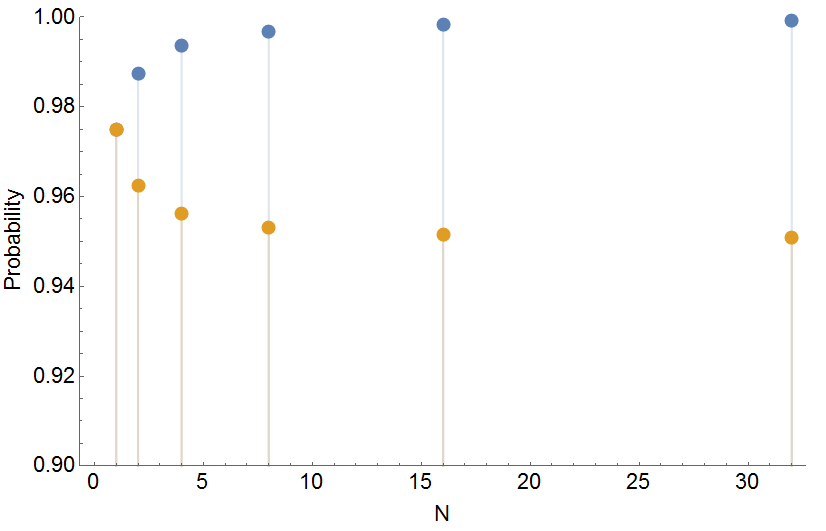
\includegraphics[width=\columnwidth]{1photonpostvsnopost.png}
	\caption{\label{fig:post vs no post} Probability of the photon being detected at the $a$ output port as shown in Figure~\ref{fig:MZ_setup} as a function of the redundant encoding size $N$. Here the phase shift noise variance was fixed at $v=0.1\ \textrm{rad}^{2}$. The lower orange values correspond to the case without post-selection and blue upper values corresponds to post-selected probability conditional on the photon not exiting the added modes in the redundant encoding.  Eq.~(\ref{eq:1pNoPost}) predicts and asymptote of $0.95$ without post-selection and Eq.~(\ref{eq:1pWithPost}) predicts an asymptote of $1$ with post-selection.}
\end{figure}

\subsection{2 photons N arbitrary \label{2 photons N arbitrary}}

The single photon interference effects in linear networks has all the features of classical wave interference.  Now we will consider two photon inference to demonstrate a truely quantum interference in this encoding.  For two photons we have a similar general form for the output state 
\begin{align}
	\left|\psi\right\rangle & =  \frac{1}{2}\left\{ 1+\frac{1}{N^{2}}\left(\sum_{j=1}^{N}\sum_{k=1}^{N}e^{i(\delta_{j}+\delta_{k})}\right)\right\} \ket{1,1} \nonumber\\
	& +\frac{\sqrt{2}}{4}\left\{ \frac{1}{N^{2}}\left(\sum_{j=1}^{N}\sum_{k=1}^{N}e^{i(\delta_{j}+\delta_{k})}\right)-1\right\} \left(\ket{2,0} +\ket{0,2}\right).\label{eq:2pNarbitrary S}
\end{align}
This equation only considers the $a$ and $b$ output modes and so includes the probability of success, as was done for the single photon case.

Here the action of the interferometer on the input state should be the identity operation and hence $\ket{1,1}$ is the desired output state.   Note that we could have chosen the input state to be $\ket{2,0}$, but this would not necessarily show any new behaviour, just the single photon results independently applied to the two input photons. 

We can again write probabilities as expectation values.  Using the form of Eq.~(\ref{eq:2pNarbitrary S}), the ideal output is achieved when
\begin{equation}
\bra{\psi}\hat{a}^{\dagger}\hat{a}\hat{b}^{\dagger}\hat{b}\ket{\psi} = 1
\end{equation}
where $\ket{\psi}$ includes any re-normalisation due to post-selection. What would will actually be achieved is
\emph{(TODO: CHECK THESE EQUATIONS)}
\begin{eqnarray}
\left\langle \psi\right|\hat{a}^{\dagger}\hat{a}\hat{b}^{\dagger}\hat{b}\left|\psi\right\rangle & = & \left\langle \left|\frac{1}{2}\left\{ 1+\frac{1}{N^{2}}\left(\sum_{j=1}^{N}\sum_{k=1}^{N}e^{i(\delta_{j}+\delta_{k})}\right)\right\} \right|^{2}\right\rangle \nonumber \\
& = & \left\langle \frac{1}{4}\left(1+\frac{2}{N^{2}}\left(\sum_{j=1}^{N}\sum_{k=1}^{N}\cos\left(\delta_{j}+\delta_{k}\right)\right)\right)\right\rangle \nonumber \\
&  & +\frac{1}{4}\Biggl\langle\frac{1}{N^{4}}\left(\sum_{j}^{N}e^{-2i\delta_{j}}+\sum_{j=1}^{N}\sum_{k\ne j}^{N}e^{-i(\delta_{j}+\delta_{k})}\right)\nonumber \\
&  & \times\left(\sum_{l}^{N}e^{2i\delta_{l}}+\sum_{l=1}^{N}\sum_{m\ne l}^{N}e^{i(\delta_{l}+\delta_{m})}\right)\Biggr\rangle\nonumber \\
& \approx & 1-v\label{eq:exp. value aabb}
\end{eqnarray}
where, a second order Taylor approximation was used along with the moments of Gaussian random variables. After post selection this is improved to become what we refer to as the probability of observing a coincidence measurement, $P(\textrm{coincidence})$, which is, to a first order approximation
\begin{widetext}
\emph{(TODO: CHECK THIS.  IT DOESN'T SEEM TO INCLUDE THE BOSONIC STATISTICS FACTOR FOR THE TWO PHOTON CASE)}
\begin{eqnarray}
P(\textrm{coincidence}) & = & \frac{\left\langle \psi\right|\hat{a}^{\dagger}\hat{a}\hat{b}^{\dagger}\hat{b}\left|\psi\right\rangle }{\left\langle \psi\right|\hat{a}^{\dagger}\hat{a}\hat{b}^{\dagger}\hat{b}\left|\psi\right\rangle +{}\left\langle \psi\right|\hat{a}^{\dagger}\hat{a}^{\dagger}\hat{a}\hat{a}\left|\psi\right\rangle +{}\left\langle \psi\right|\hat{b}^{\dagger}\hat{b}^{\dagger}\hat{b}\hat{b}\left|\psi\right\rangle }\nonumber \\
& \approx & 1-\frac{v}{2N}\label{eq:2pNarb PS}
\end{eqnarray}
\end{widetext}
where the binomial approximation was also used.  Finally the probability of success, when defined as the probability of not needing to post selected a single instance is
\begin{eqnarray}
	P(\textrm{success}) & \approx & 1-v+\frac{v}{2N}.\label{eq:2pNarb Success}
\end{eqnarray}

Here, again in the large $N$ limit the result matches Equation \ref{eq:Gaussian Psuccess} provided it is squared before taking the linear approximation. Also both these instances we see the probability of success scaling with $\frac{1}{N}$.

\section{Comparison between averaging techniques \label{averaging at end vs step}}

So far we have presented two specific procedures for implementing a redundantly encoded phase shift with linear elements.  There exists many more combinations of possible ways to do this.  In this section we will look at combinations of redundant encodings using the concatenated beam-splitter method.  In particular we will study two different methods, which we will referred to as averaging at the end and averaging each step. Figure \ref{fig:Different methods of implementation} shows schematically these two configurations.  By averaging each component individually (Fig.~\ref{fig:Different methods of implementation}(c)), significantly more encoding resources are required, however we will show this leads to more stability in the output state. In the low resource and low error limit these two methods also appear to be directly equivalent. We can then infer that in the case when the two methods do yield equivalent results, Corollary \ref{Corollary 2}, and its approximately commuting error assumption, does hold. In particular the low error limit allows the approximation that the generators of each error commute with one another. However this approximately commuting assumption will fail to hold in general when the size of the errors becomes too large. The effect of this can lead to significant differences in the effectiveness of the two arrangements as discussed in this section.
\begin{figure}
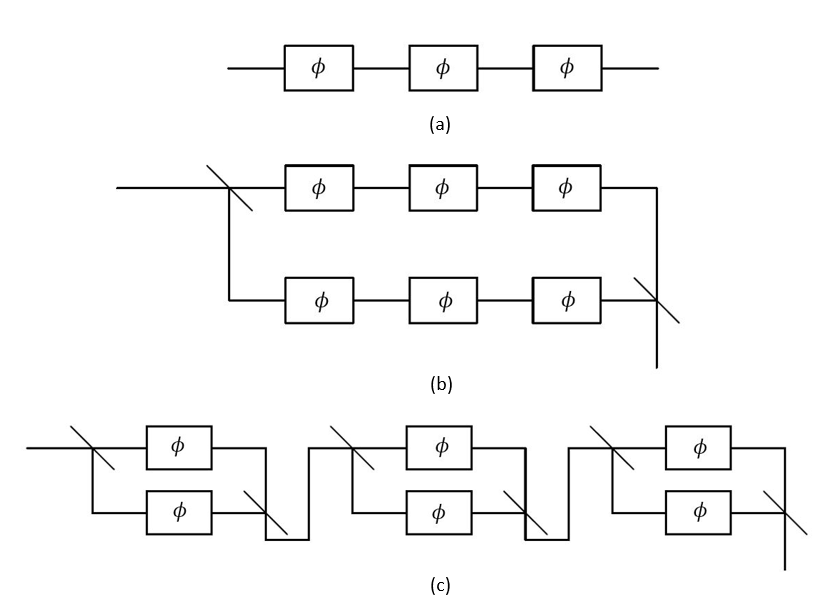
\includegraphics[width=\columnwidth]{three_phase_applying_systems.PNG}
\caption{Three methods of applying three phase shifts, each marked with a in
	series. (a) Three phase shifts with no error averaging. (b) Three phase
	shifts when averaging across the system. (c) Three phase shifts when
	averaging across each phase shifter individually. Averaging across the
	system will in general require far fewer encoding resources.
	\label{fig:Different methods of implementation}}
\end{figure}

\subsection{Phase applying systems\label{Phase applying systems}}
For a more complete picture, this section considers the output of a simple phase applying system on a `shot by shot' case as well as expectation values. This will also serve to highlight the differences between the two implementations.

In this section Error Averaging after each applied phase shift is compared to averaging across the entire system. The system was analysed contains a single channel with $m$ sequential phase shifters. This was chosen to better characterise Error Averaging when applied to a series of error sources as any differences between the two methods of error correction will be more likely arise in larger systems. This allows us to see the effect of having multiple parameters in a single mode and so the results should be governed by Corollary \ref{Corollary 1}. These systems were also used to determine if a quantum Zeno effect  \cite{expZeno} also known as the Turing paradox would be observed.

Figure \ref{fig:Different methods of implementation} shows the set-up for the phase applying systems.

Following a very similar approach to the earlier sections, for the sake of generating meaningful expectation values, the applied phase shifters were placed in one arm of a MZ interferometer. The one photon number expectation values can thus be calculated. For simplicity the applied phase shift was chosen to be zero with a Gaussian random noise with a variance $v$. This was chosen such that the errors here match what was modelled in sections \ref{1 photon N arbitrary} and \ref{2 photons N arbitrary}. The probability of success is now defined as the photon number expectation value evaluated at the end of the phase applying systems while the strength of the error was initially defined as the photon number expectation value of the MZ interferometer system for the expected output had no error occurred. All approximate results are based of fourth order Taylor approximations with comparisons drawn to the second order approximations as used in previous sections. This system corresponds to the chaining together of Equation \ref{eq:single parameter, multi-mode} with 
\begin{equation}
T=\begin{bmatrix}
	0 & 1 \\
	1 & 0 \\
	\end{bmatrix}
\end{equation}

\subsubsection{No Averaging\label{No Averaging}}

Starting with the baseline comparison case, seen in Figure \ref{fig:Different methods of implementation}a, where no Error Averaging is used, the output state for a single photon going through just the phase applying system will simply be
\begin{equation}
\left|\psi\right\rangle =\left(\prod_{k=1}^{M}e^{i\delta_{k}}\right)\left|1\right\rangle \label{eq:noAvPhaseState}
\end{equation}
The probability of success is then
\begin{eqnarray}
P\left(success\right) & = & \left\langle \psi|\psi\right\rangle \nonumber \\
& = & \left\langle 1\right|\left(\prod_{l=1}^{M}e^{-i\delta_{l}}\right)\left(\prod_{k=1}^{M}e^{i\delta_{k}}\right)\left|1\right\rangle \nonumber \\
& = & 1\label{eq:noAveProbSuccess}
\end{eqnarray}
which is unsurprising given there is no way, ignoring losses, for the photon to leave this particular system.

To determine a measure of the error the phase applying system was then inserted into a MZ interferometer giving a total output state $\ket{\Psi}$. The error is then determined by considering the photon expectation value in the correct output mode with post selection. As however the probability of success is unity no post selection will occur. So the output state is
\begin{equation}
\left|\Psi\right\rangle =\frac{1}{2}\left(\prod_{k=1}^{M}e^{i\delta_{k}}+1\right)\hat{a}^{\dagger}\left|0\right\rangle +\left(\prod_{k=1}^{M}e^{i\delta_{k}}-1\right)\hat{b}^{\dagger}\left|0\right\rangle \label{eq:noAveIntState}
\end{equation}
Now our error measure when no averaging is applied, $E_{noAv}$, will be
\begin{eqnarray}
E_{noAve} & = & \left\langle \Psi\right|\hat{n}_{a}\left|\Psi\right\rangle \nonumber \\
& = & \frac{1}{2}\left\langle 1+\cos\left(\alpha\right)\right\rangle \nonumber \\
& \approx & 1-\frac{Mv}{4}+\frac{M^{2}v}{16}\label{eq:ErrorNoAv1}
\end{eqnarray}
Where Gaussian statistics have been used to write higher order moments in terms of the variance.

\subsubsection{Averaging Across the Entire Phase System\label{Averaging Across the Entire Phase System}}

We now consider averaging across the whole system, as shown in Figure  \ref{fig:Different methods of implementation}b. Preceding as before, the state for a single photon after passing through the phase applying system which is being averaged across will simply be
\begin{equation}
\left|\psi\right\rangle =\frac{1}{N}\sum_{j=1}^{N}\left(\prod_{k=1}^{M}e^{i\delta_{j,k}}\right)\left|1\right\rangle \label{eq:AvEndPhaseState}
\end{equation}
The probability of success is thus
\begin{eqnarray}
P\left(success\right) & = & \left\langle \psi|\psi\right\rangle \nonumber \\
& \approx & \left[1-\left(1-\frac{1}{N}\right)\left(Mv-\frac{1}{2}M^{2}v^{2}\right)\right]\label{eq:AveEndProbSuccess}
\end{eqnarray}
This result is similar to the what was found in previous sections, see Eq.\ref{eq:1pNarbitrary successs} and Eq.\ref{eq:2pNarb Success}, with the probability of success asymptotically approaching some fixed value for large $N$.

To determine the size of the error, the phase applying system was again inserted into the phase arm of a MZ interferometer giving a total output state $\left|\Psi\right\rangle $. The error is then given by the photon expectation value in the correct output mode with post selection. The output state is
\begin{eqnarray}
\left|\Psi\right\rangle & = &\frac{1}{2}\left(\frac{1}{N}\sum_{j=1}^{N}\left(\prod_{k=1}^{M}e^{i\delta_{j,k}}\right)+1\right)\hat{a}^{\dagger}\left|0\right\rangle \\ & & +\left(\frac{1}{N}\sum_{j=1}^{N}\left(\prod_{k=1}^{M}e^{i\delta_{j,k}}\right)-1\right)\hat{b}^{\dagger}\left|0\right\rangle \label{eq:AveEndIntState}
\end{eqnarray}
So the photon number expectation value for the correct output for this system will be
\begin{widetext}
\begin{eqnarray}
\left\langle \Psi\right|\hat{n}_{a}\left|\Psi\right\rangle  
& \approx & 1-\frac{1}{4}\left(Mv-\frac{M^{2}v^{2}}{4}+\left(1-\frac{1}{N}\right)\left(Mv-\frac{1}{2}M^{2}v^{2}\right)\right)
\end{eqnarray}
Similarly for the incorrect output port, the photon number expectation value will be
\begin{equation}
\left\langle \Psi\right|\hat{n}_{b}\left|\Psi\right\rangle = \frac{1}{4}\left\langle 1+\left\langle \psi|\psi\right\rangle -\frac{2}{N}\sum_{j=1}^{N}\cos\left(\alpha_{j}\right)\right\rangle 
\end{equation}
Therefore, the error measure, $E_{aveEnd}$, will be
\begin{equation}
E_{aveEnd}  \approx  \left[1-\frac{1}{4}\left(Mv-\frac{M^{2}v^{2}}{4}+\left(1-\frac{1}{N}\right)\left(Mv-\frac{1}{2}M^{2}v^{2}\right)\right)\right]\nonumber\times\left[1-\left(1-\frac{1}{N}\right)\left(\frac{Mv}{2}-\frac{1}{4}M^{2}v^{2}\right)\right]^{-1}\label{eq:ErrorAvEnd}
\end{equation}
\end{widetext}

\subsubsection{Averaging Across Each Phase Shifter Individually\label{Averaging Across Each Phase Shifter Individually}}

If each phase shifter is averaged individually, as seen in Figure \ref{fig:Different methods of implementation}c, then the state for a single photon after passing through the phase applying system will be
\begin{equation}
\left|\psi\right\rangle =\frac{1}{N}\prod_{k=1}^{M}\left(\sum_{j=1}^{N}e^{i\delta_{j,k}}\right)\left|1\right\rangle \label{eq:AveStepPhaseState}
\end{equation}
Reproducing the above calculations with this state yields a probability of success of
\begin{equation}
P\left(Success\right)\approx\left(1-\left(v-\frac{v^{2}}{2}\right)\left(1-\frac{1}{N}\right)\right)^{M}\label{eq:AvStepProbSuccess}
\end{equation}
and an error of
\begin{widetext}
\begin{equation}
E_{aveStep} \approx  \left[\frac{3}{4}-\frac{Mv}{4}+\frac{M^{2}v^{2}}{16}+\frac{1}{4}\left(1-\left(v-\frac{v^{2}}{2}\right)\left(1-\frac{1}{N}\right)\right)^{M}\right]\nonumber\times\left[\frac{1}{2}+\frac{1}{2}\left(1-\left(v-\frac{v^{2}}{2}\right)\left(1-\frac{1}{N}\right)\right)^{M}\right]^{-1}\label{eq:ErrorAvStep}
\end{equation}
\end{widetext}
Importantly, for both this case as well as when averaging each step, if only the first order approximation is used and $M=1$ then the error matches the error found in section \ref{1 photon N arbitrary}. This is simply highlighting that Error Averaging scales in a very predictable manner.

\subsubsection{Summary of Errors and Probabilities\label{Summary of Errors and Probabilities}}

Figure \ref{fig:Error-as-measured all} shows how the error, as measured by looking at expected photon number values in the output port of a MZ interferometer, varies as the number of phase components increases as well as how the error changes with increasing Error Averaging, $N$. The behaviour as $N$ increases is as expected with the error close to disappearing for low $M$, that is, a small number of phase shifters in series, and $N=16$. Interestingly a difference between the two Error Averaging methods can be seen from $M\approx6$ onwards. This could either be suggesting an issue with the quality of the second order approximations, as seen in Figure \ref{fig:Probability-of-success all} or that there is some more fundamental point at which there is a clear benefit to averaging each component individually. The next consideration was how the probability of success changes with $M$.

\begin{figure}
\centerline{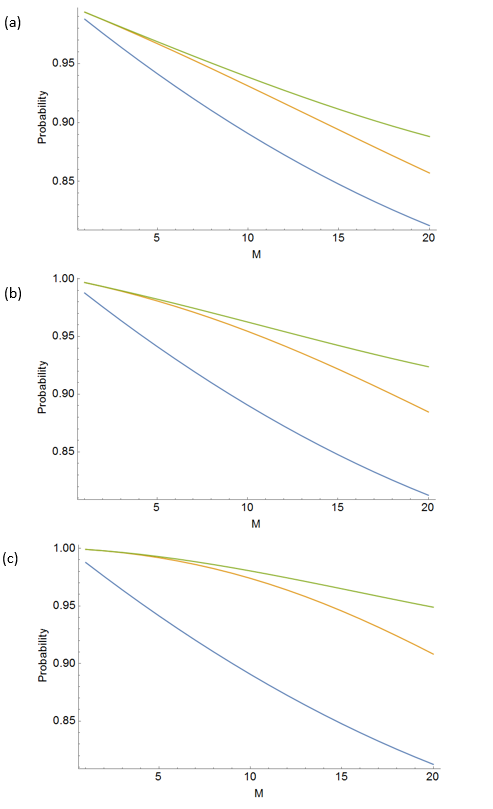
\includegraphics[width=\columnwidth]{Error_all.png}}
\caption{Probability of obtaining the correct result as measured by the Mach Zehnder interferometer set up as a function of the number of phase components $M$. Here a probability of $1$ corresponds to no error and the smaller the probability the larger the error. The blue line represents the no Error Averaging applied result, the orange line corresponds to the error when averaging across the entire system and the green line is the error when each component is averaged across individually. All three graphs were created with the variance of the error in a single phase shifter being $0.005\ \textrm{rad}^{2}$ and for a) $N=2$, in b) $N=4$ and in c) $N=16$. \label{fig:Error-as-measured all}}
\end{figure}
Figure \ref{fig:Probability-of-success all} shows how the probability of success changes as the number of phase shifters in a series increases when averaging across the entire system as well as when averaging across each component individually. The effect of varying the amount of averaging is also shown. A first and second order analytical solutions	is  shown as well as a statistical model of the probability of success where the phase value of each phase shifter was sampled from a Gaussian random distribution. The probability of success was then calculated based on these random samples. The top four graphs were plotted for an unrealistically low value of the variance on the individual beam splitters. This was done so that the behaviour of when the first and second order approximations fail to match the actual simulated result can be more clearly seen. 

It is seen that as the total number of components increases the probability of success decreases. However it does so at a decreasing rate which is important for scaling to large systems. The two methods of Error Averaging also show very similar behaviour in their overall trends although the variation between the statistical simulation and the analytical solutions is significantly greater when averaging across the entire system than when averaging each component individually. This is suggestive of a manifestation of the Zeno effect, whereby continuously correcting produces less variation than doing the same amount of correction at the end. First and second order solutions in the averaging over the entire system case fail very early when compared with those for averaging every step. Interestingly it appears that the first order analytical approximation is suitable when averaging each component individually. This can most clearly be seen in Figure \ref{fig:Probability-of-success all} (e) where the first order approximation fails almost instantly and the second order approximation soon after while in Figure \ref{fig:Probability-of-success all} (f) both first and second order approximations both follow the statistical model closely. It is again observed that as $N$ increases, the probability of success goes down. What is also shown however is that so too does the variation in the statistical simulation suggesting greater amount of averaging reduces the variability in both the average case and any given sample of the applied phase.

\begin{figure}
\centerline{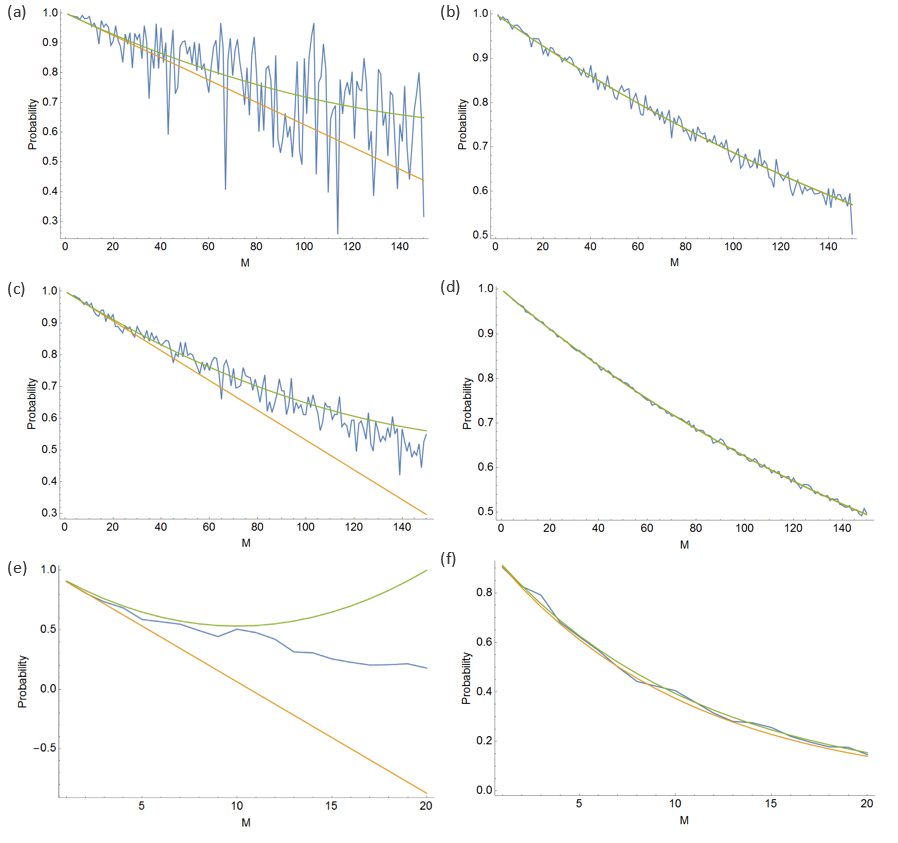
\includegraphics[width=\columnwidth]{Psuccess_all.png}}
\caption{Probability of success as a function of the number of phase components $M$ for averaging across the system (left) and averaging across each component (right). Blue line is the statistical model, orange is the first order approximation and green is the second order approximation of the analytical value. a) and b) individual phase shifter variance is $0.005\ \textrm{rad}^{2}$ with $N=4$, c) and d) individual phase shifter variance is $0.005\ \textrm{rad}^{2}$ with $N=16$ and e) and f) individual phase shifter variance is $0.1\ \textrm{rad}^{2}$ with $N=16$. \label{fig:Probability-of-success all}}
\end{figure}

To gain a better insight into how the error behaves and what the difference between the two averaging methods actually is, the actual phase being applied with each system was modelled, as discussed in the following subsection.


\subsubsection{Statistical Modelling of the Applied Phase\label{Statistical Modelling of the Applied Phase}}

To better understand the behaviour of the three phase applying systems, the total applied phase was modelled using \textit{Mathematica} with phase values chosen from a Gaussian random distribution with mean $0$ and variance $v$. This now corresponds to Equation \ref{eq:single parameter, single mode} with $\theta=\prod_{i}\theta_{i}$. This was repeated $5000$ times and the results are shown in Figure \ref{fig:Total-applied-phase1} and Figure \ref{fig:Total-applied-phase2}. This again shows a difference between averaging across the entire system and averaging at each step. In particular the range of applied phases is noticeably smaller when each phase shifter is corrected individually, a clear indication that averaging each step is more effective. By comparing Figure \ref{fig:Total-applied-phase1} with Figure \ref{fig:Error-as-measured all} at $M=15$ we can infer that the difference between the two error correction methods seen in Figure \ref{fig:Error-as-measured all} is not entirely due to the quality of the approximations used in each case. In particular we can infer that the region in which the two methods give the same results corresponds to the region in which the $u(n)$ errors approximately commute with one another and are therefore separable.

\begin{figure}
\centerline{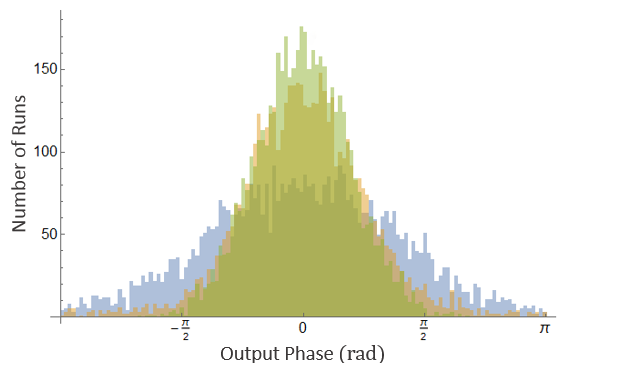
\includegraphics[width=\columnwidth]{totPhase1.png}}
\caption{Top: Total applied phase over $5000$ runs for no averaging (Blue), averaging across the entire system (Orange) and averaging each phase shifter individually (Green). Bottom: Histogram of the total applied phases. Each individual phase shifter has a variance of $0.1\ \textrm{rad}^{2}$ and each system has $15$ phase shifters in series. The two error averaged circuits are each averaged $4$ times. \label{fig:Total-applied-phase1}}
\end{figure}

\begin{figure}
\centerline{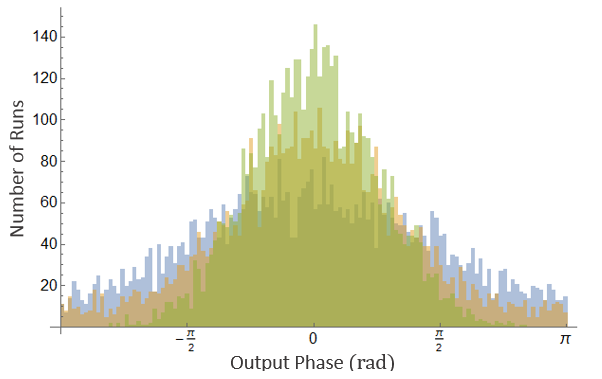
\includegraphics[width=\columnwidth]{totPhase2.png}}
\caption{Top: Total applied phase over $5000$ runs for no averaging (Blue), averaging across the entire system (Orange) and averaging each phase shifter individually (Green). Bottom: Histogram of the total applied phase. Each individual phase shifter has a variance of $0.3\ \textrm{rad}^{2}$ and each system has $8$ phase shifters in series. The two error averaged circuits are each averaged $4$ times. \label{fig:Total-applied-phase2}}
\end{figure}

To further investigate this behaviour the variance of the applied phase was calculated based on the statistical simulation of the total applied phase. This was then plotted as a function of $M$, the number of phase shifters in a series as shown in Figure \ref{fig:Variance-in-phase all}. Given the individual applied phase are Gaussian random variables they are expected to simply add, such that the variance without any Error Averaging is expected to simply be
\begin{equation}
\textrm{Total Variance}=vM\label{eq:Tot Var no correction}
\end{equation}
where $M$ is the number of phase shifters and $v$ is the variance in the individual phase shifter. The total variance when Error Averaging can similarly be expected to simply be
\begin{equation}
\textrm{Total Variance}=\frac{vM}{N}\label{eq:Tot Var w/ correction}
\end{equation}
where $N$ is the number of times the system is averaged, again $N=1$ implies no averaging. As the phase is an angle this behaviour cannot hold for arbitrarily large $vM$. A completely random phase $\theta$ is still limited by the possibly range of values, in our case chosen to be $-\pi<\theta\le\pi$. If the value of $\theta$ is indeed completely random then one will expect a uniform probability distribution of $P\left(\theta\right)=\frac{1}{2\pi}$. 

This then implies the maximum variance will be given by
\begin{eqnarray}
\textrm{Maximum variance} & = & \int_{-\pi}^{\pi}\theta^{2}P\left(\theta\right)\ d\theta\nonumber \\
& = & \frac{\pi^{2}}{3}\label{eq:Max Var}
\end{eqnarray}

\begin{figure}
\centerline{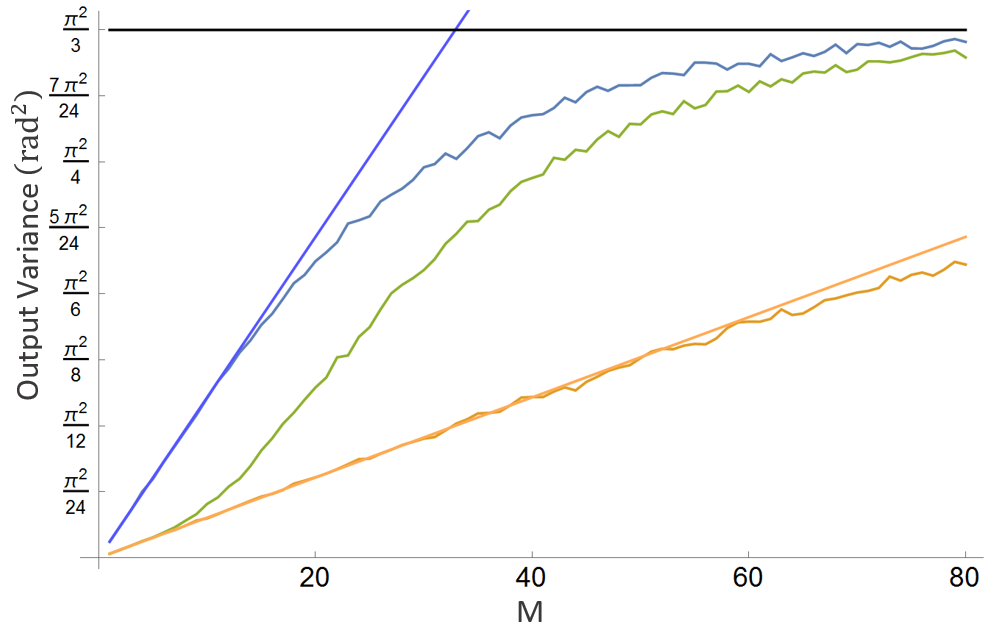
\includegraphics[width=\columnwidth]{phase_all.png}}
\caption{Variance in the total applied phase without Error Averaging (Blue), when averaging across the entire system (Green) and when averaging each component individually (Orange), all plotted as a function of the number of phase shifters in series $(M)$. The variance of a single phase shifter is $0.1\ \textrm{rad}^{2}$ and the two error averaged systems averaged 4 times. The predicted, linear variance without any averaging (lighter blue) and with averaging (lighter orange) is also shown. These ignore the fact that the variance is actually the angular variance and so has some maximum allowable value given by Eq. \ref{eq:Max Var}, which is also shown in black. \label{fig:Variance-in-phase all}}
\end{figure}


Figure \ref{fig:Variance-in-phase all} shows that the two methods of error correction do indeed initially have the same effect. However the averaging across the system method falls out of this linear regime from approximately $M=6$ after which it follows the general form of applying no correction. This suggests this corresponds to the point at which all errors cannot be assumed to approximately commute. The fact that averaging across the entire system mirrors the no averaging trend suggest that the positive effects of Error Averaging completely disappear in this regime. Averaging each step however does not appear to fall out of the linear regime. The down turn at higher total output variance can be attributed to the variance approaching the maximum possible variance and so any behaviour in this region can be considered insignificant as the output results generated from a system in this regime is likely to be quite random. To determine if and when the averaging each step method of error correction fails this process was repeated, now as a function of the variance in a single beam splitter. The total variance was determined from $50000$ data points for each value of $v$. Figure \ref{fig:Variance(veriance)} demonstrated that again the two error correction methods initially are equivalent. Once more averaging across the system falls out of the linear regime and now we can clearly see so too does the averaging each step.

This is highly suggestive of the existence of some threshold for the amount of error in a system before Error Averaging fails to be beneficial. It also suggests this threshold might correspond to when the errors no longer approximately commute. A single phase shifter with variance $v_{1}$ is effectively equivalent to $m$ phase shifters with individual variance $v_{2}=\frac{v_{1}}{m}$ if the entire system is being averaged across. This allows the phase error threshold to be estimated at about $0.5\ \textrm{rad}^{2}$when averaging across each element and $\frac{0.5}{m}\textrm{rad}^{2}$ when averaging across a system of $m$ phase shifters. If each individual beam splitter has a variance of $0.1\ \textrm{rad}^{2}$, averaging across the system would be expected to be in the linear regime when $M\le5$ which is precisely what is seen in Figure \ref{fig:Variance-in-phase all}. These two thresholds obviously do not apply to a general error however it is hoped that with further study might reveal the values for such a threshold.
\begin{figure}
\centerline{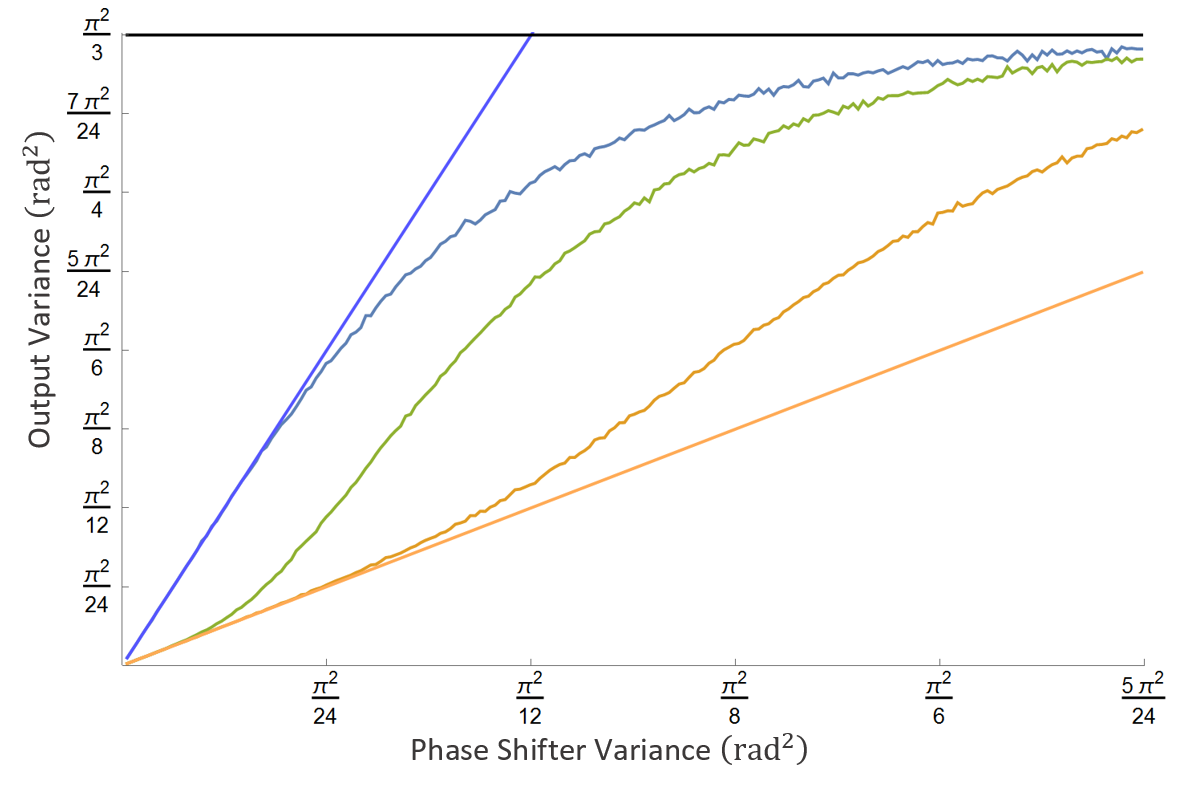
\includegraphics[width=\columnwidth]{variance(variance).png}}
\caption{Variance in the total applied phase without Error Averaging (Blue), when averaging across the entire system (Green) and when averaging each component individually (Orange), all plotted as a function of the variance in each individual phase shifter. Each system applied $4$ phase shifters in series, that is $M=4$, and the two error averaged systems averaged $4$ times, that is $N=4$. The predicted variance without any averaging (lighter blue) and with averaging (lighter orange) is also shown along with the maximum allowable variance. \label{fig:Variance(veriance)}}
\end{figure}

It can now be concluded that some hybrid method of Error Averaging would be most suitable in general. The entire system would need to be broken into $x$ smaller systems, which are independently averaged across. The specific value of $x$ would be such that the number of components in the system, $m$, is maximised while the total error within each subsystem is kept below the appropriate threshold.

\subsection{Four Mode Implementation Comparison \label{Four Mode Impementation Comparison}}

To gain a better understanding of how useful this method of Error Averaging actually is, a more complicated system was also investigated. In particular, a four mode system with each method of Error Averaging was considered. The set up consisted of a four mode system with four beam splitters, each implemented as above, that is each being its own MZ interferometer as shown in Figure \ref{fig:4 mode basis diagram}. Three different input states were chosen: a single photon input in the top mode and the vacuum state at all other modes$\left(\left|1,0,0,0\right\rangle \right)$, two photons, both in the top mode $\left(\left|2,0,0,0\right\rangle \right)$ and two photons spread across the top two modes $\left(\left|1,1,0,0\right\rangle \right)$. For simplicity the system was chosen to target the identity and error reduction was then applied using both implementations. That is, by averaging each beam splitter as done in section \ref{1 photon N arbitrary} and by concatenating the entire system in an interferometer as shown in Figure \ref{fig: averaging 4 mode diagram}. All results were found using \textit{Mathemtatica} to sample from the appropriate transformation matrix representing the system and then compute the second order approximation of the photon number expectation values and probabilities for $N=1, 2 \textrm{ and } 4$. All results can be found in Appendix \ref{Appendix full of results}

\begin{figure}[h]
\centerline{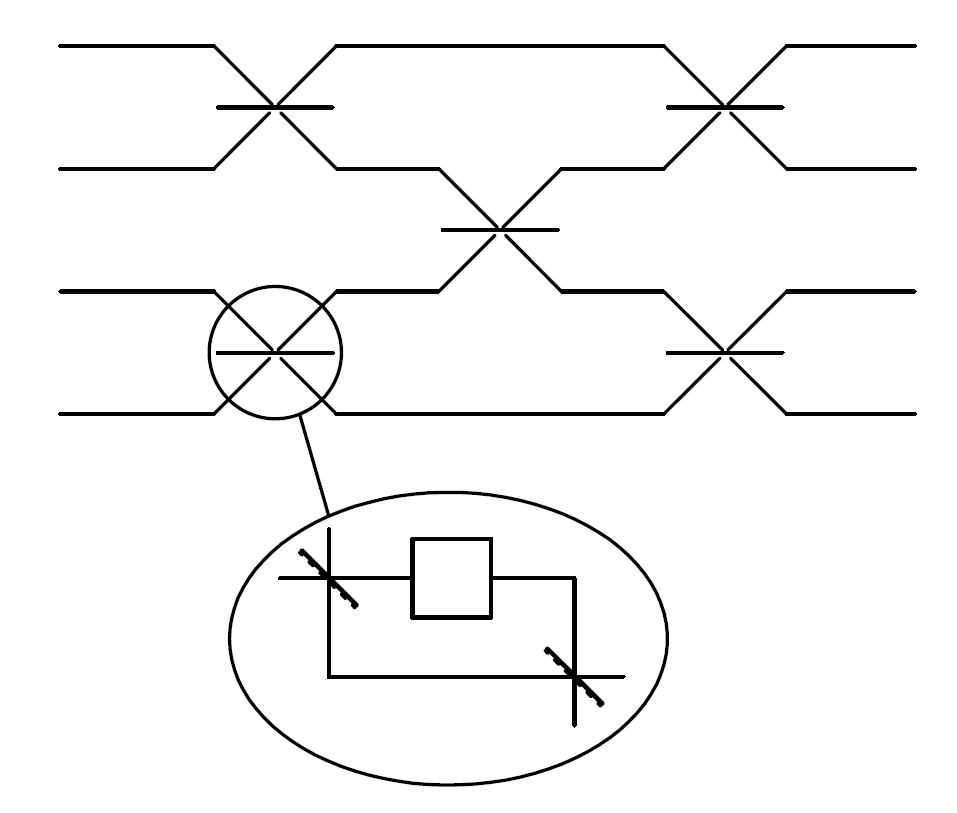
\includegraphics[width=\columnwidth]{4_mode_N=2.jpg}}
\caption{Diagram of the four mode linear optical network which forms the basis of the four mode set-ups. \label{fig:4 mode basis diagram}}
\end{figure}

\begin{figure}[h]
\centerline{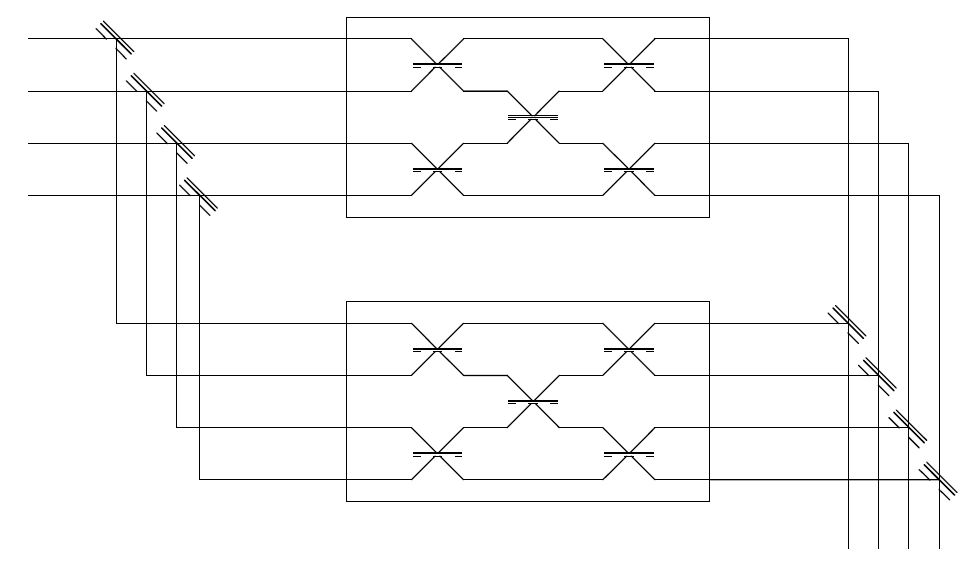
\includegraphics[width=\columnwidth]{4_mode_average_across.jpg}}
\caption{Diagram of the four mode linear optical network averaged across the system once. A two mode system averaged in this fashion could be considered as an Error Averaged dual rail single qubit unitary transformation. \label{fig: averaging 4 mode diagram}}
\end{figure}

After determining the output probability distribution with and without post selection it was found that the two correction methods produced equivalent results. The $1/N$ scaling in error after post selection, as seen above, was also observed, suggesting this pattern holds for an arbitrary number of modes and arbitrary system. The following section is based on the results of these simulations.

\subsubsection{Generalising Example Results}

Starting with no error reduction, and given the correct output state $\left|\psi\right\rangle $ the following sequence can be defined. First defining the probability of obtaining the correct result as when $N=1$:
\begin{equation}
P_{1}(correct)=1-\frac{a_{1}}{b_{1}}v
\end{equation}
The probability of an incorrect state is therefore trivially:
\begin{equation}
P_{1}(wrong)=\frac{a_{1}}{b_{1}}v
\end{equation}
At this stage there are no error ports and so $P_{i}(wrong)+P_{i}(correct)$	represents the probability of success as previously defined. Note that the subscript indexes the corresponding size of the system. Explicitly $i+1$ corresponds to a system with twice as much averaging as $i$.
So averaging once changes these values to:
\begin{eqnarray}
P_{2}(correct) & = & 1-\frac{2a_{1}+1}{2b_{1}}v\nonumber \\
& \equiv & 1-\frac{a_{2}}{b_{2}}v
\end{eqnarray}
\begin{eqnarray}
P_{2}(wrong) & = & \frac{a_{1}}{2b_{1}}v\nonumber \\
& \equiv & \frac{a_{2}}{b_{2}}v
\end{eqnarray}
And so on, so in general:
\begin{eqnarray}
P_{n}(correct) & = & 1-\frac{2a_{n-1}+1}{2b_{n-1}}v\nonumber \\
& = & 1-\frac{\left(2^{n-1}a_{1}+\left(2^{n-1}-1\right)\right)}{2^{n-1}b_{1}}v\\
P_{n}(wrong) & = & \frac{a_{n-1}}{2b_{n-1}}v\nonumber \\
& = & \frac{a_{1}}{2^{n-1}b_{1}}v
\end{eqnarray}
The probability of getting the correct state with post selection will then be
\begin{eqnarray}
&  & P_{n}\left(correct\left|\textrm{post selection}\right.\right)\nonumber \\
& = & \left(1-\frac{a_{1}}{2^{n-1}b_{1}}v\right)\xrightarrow[n\rightarrow\infty]{}1\label{eq:PcorrectGeneral}
\end{eqnarray}
The probability of success was found to be
\begin{equation}
P_{n}\left(success\right) =  1-\frac{\left(2^{n-1}-1\right)\left(a_{1}+1\right)}{2^{n-1}b_{1}}v\nonumber \\
\end{equation}
Hence we get a general bound on the probability of success as
\begin{equation}
\lim_{n\rightarrow\infty}P_{n}\left(success\right)=1-\left(\frac{a_{1}+1}{b_{1}}\right)v\label{eq:PsuccessGeneral}
\end{equation}
The equivalence of the two methods of implementation suggest that all results were once again taken from the regime where all errors approximately commute. The result can also be understood to be the first order approximation to Equation \ref{eq:approx commuting, general case}. The $\frac{a_1+1}{b_1}$ coefficient does not quite match what might be expected from Equation \ref{eq:approx commuting, general case} however it can be understood as a result of commuting all errors past the target unitary. Another possible explanation is that there not any clear isomorphic map between the parameters in the system and the error coefficients of the Lie algebra generators.

This result hints at the self correcting nature of Error Averaging. By considering the inner corrected system with error laden beam splitters as the initial step in the sequence then each further step will be averaging across both the fixed beam splitters and the original error laden system. This could allow some of the beam splitters to be corrected  making the base assumptions on the quality of the fixed beam splitters less restrictive. This is highlighted in Figure \ref{fig:gen system} where, depending on which components are considered to be the system, it is averaged either $8$, $4$ or $2$ times. 

\section{Feasibility of Error Averaging\label{Feasibility section}}

\subsection{A Short Note on Boson Sampling\label{Boson Sampling}}

Having achieved some semi-general results in terms of what benefit can be obtained from Error Averaging, the next question which arises is; when is it useful? All previous results suggest that Error Averaging, in its current state, is particularly useful for any system in which the result cannot simply be checked to verify the results. This is concluded as Error Averaging trades certainty in obtaining some results with certainty in the quality of the result obtained. The question still remains of how best to implement Error Averaging. In particular, how to minimise the number of encoding resources while ensuring the system remains in the approximately commuting regime.

To explore this, a general $m$ mode system is considered. It would be constructed such that each input mode is connected to each output mode and every path will have the same number of beam splitters and phase shifters. The first requirement was for the system to be considered in some sense general. Note that this system while being general in that every mode will be mixed with every other mode, the system is insufficient to implement an arbitrary unitary transformation of the input. The second requirement, that each path has the same number of beam splitters and phase shifters to ensure the system's error profile is completely symmetric.

To create such a system it was decided to require $m$ to be even and arrange the beam splitters in columns with $b=\frac{m}{2}$ beam splitters in each column. They are arranged such that, starting with the top most mode, the first column mixes nearest neighbour modes, the second column mixes the next nearest neighbour modes and each subsequent column mixes the next closest mode which it is yet to be mixed with. This gives a depth of $c$ columns where $c=\left\lceil \log_{2}(m)\right\rceil $.

This system as it currently stands is not suitable for implementing an arbitrary unitary transformation. This is known because for a system to be suitable to simulate $\mathfrak{U\mathrm{(m)}}$, it must have on the order of $O\left(m^{2}\right)$ beam splitters and phase shifters \cite{reck}. This system however only has
\begin{equation}
b\times c=\frac{m}{2}\log_{2}(m)
\end{equation}
beam splitters and so, if each beam splitter has a single phase shifter than the number of controllable components will be $m\log_{2}(m)$ rather than the necessary $O\left(m^{2}\right)$. Using such a system we can either average across the system or average each component individually to protect against errors.

To determine the feasibility and usefulness of Error Averaging it is necessary to determine what circumstances the assumption which has been made is valid. Namely the assumption that perfect, fixed $50:50$ beam splitters can be used to build the averaging circuit. The following discussion ignores the probability of success of Error Averaging, which will lead to an exponential overhead in the number of times the device must be run before obtaining a successful outcome. To address this Error Averaging will require a loss recovery code \cite{OQC} however this is outside the scope the current paper. At this point it is worth noting that in the paper  \textit{Universal Linear Optics} a single, controllable, beam splitter was implemented using the same Mach-Zehnder interferometer set-up discussed previously with fidelity $\mathcal{F}=0.992\pm0.008$ \cite{ULO}. 

This is useful to consider as it suggests that currently we can have quite high quality, low error components. One necessary and perhaps sufficient condition for this assumption to be valid is for the number of error causing components in the system to be far greater than the number of perfect components required. This would imply that even if the fixed beam splitters are no better than the variable ones being implemented, Error Averaging will still dramatically reduce the total error in the system. 

It is known \cite{reck} that a system requires $O\left(m^{2}\right)$ controllable components to be sufficient to implement $\mathfrak{U}\left(m\right)$. If such a system is corrected using Error Averaging and the minimum number of correction components then the method of correcting across the entire system would be used. To average a single mode $N$ times, $2\left(N-1\right)$ perfect beam splitters are required. So the precise resource cost will be dependent on the circuits specific set-up. Following on from the previously described set up, we know we can mix $m$ modes in a unique way such that every path has the same number of beam splitters and phase shifters with a circuit depth of $\log_{2}\left(m\right)$. Aaronson and Arkhipov, inspired by a boson sampling type system with $n$ photons in the top $n$ modes, have shown \cite{Boson} that for this system to be adequate to implement an arbitrary unitary operation it must be chained together $n$ times. Each block will have $m$ modes, a depth of $\log_{2}\left(m\right)$ and therefore $\frac{m}{2}\log_{2}\left(m\right)$ beam splitters. This then means that our system will have $\frac{mn}{2}\log_{2}\left(m\right)$ error laden components and require a minimum of $2\left(N-1\right)m$ correction components to allow for averaging $N$ times across the entire system. Given that averaging across the entire system falls out of the linear regime very quickly as the depth increases it would likely be insufficient to correct our system. If however each component has Error Averaging applied to it individually then there would need to be at most $mn\log_{2}\left(m\right)\left(N-1\right)$ perfect $50:50$ beam splitters, more than the original size of the circuit. Note this can result in correcting components which cannot possibly be involved in the result. For example if only the top one or two modes have photon inputs then only $2\left(m-1\right)\left(N-1\right)+m\left(n-1\right)\log_{2}\left(m\right)\left(N-1\right)$ correction components are necessary. The upper bound on the number of correction components, $mn\log_{2}\left(m\right)\left(N-1\right)$, is more general, and so will be used for the remainder of this discussion. This suggests something part way between these two cases is necessary. If a system was split up into $x$ sections, each of which is averaged $N$ times, than $2xm\left(N-1\right)$ correction components are necessary. This then gives the very loose inequality of
\begin{eqnarray}
2xm\left(N-1\right) & \ll & \frac{mn}{2}\log_{2}\left(m\right)\nonumber \\
4x\left(N-1\right) & \ll & n\log_{2}\left(m\right)\label{eq:veryLooseInequality}
\end{eqnarray}


for the assumption that an averaging circuit can be made using relatively perfect beam splitters to be valid. The requirement of Error Averaging to be in the linear regime will also impose the condition that $x\rightarrow n\log_{2}\left(m\right)$ as the error in each component gets bigger. There is the possibility that this is not quite so bad however as most of the perfect beam splitters are actually error averaged themselves as shown in Figure \ref{fig:gen system}. This could allow greater freedom in what is meant by a perfect beam splitter. However even if only the outermost beam splitters are to be considered, and all inner beam splitters are said to be corrected themselves, there will still require between $2m$ and $mn\log_{2}\left(m\right)$ perfect fixed beam splitters.

Another important issue is to decide how any times the system needs to be averaged, that is, how $N$ needs to grow with $m$ and $n$. It has been shown that for the total systems error to be vanishingly small the error in each individual element in a linear optical system needs to be on the order of $\frac{1}{n}$ where $n$ is the number of photons \cite{arkhipov2014}. It has also been shown that it is necessary for the error to scale as $\frac{1}{n\log_{2}\left(m\right)}$ \cite{Boson} in the case of a boson sampling style system with $1$ photon in the first $n$ modes of an $m$ mode system. Combining these two results gives a necessary scaling of $\frac{1}{n^{2}\log_{2}\left(m\right)}$. All of our results so far suggest the error scales as $\frac{1}{N}$. By using this scaling we can estimate that $N\sim n^{2}\log_{2}\left(m\right)$ for the total error in the output to be preserved. Combining this with Eq. \ref{eq:veryLooseInequality} then gives
\begin{equation}
4x\left(n^{2}\log_{2}\left(m\right)-1\right)\ll n\log_{2}\left(m\right)\label{eq:LooseInequality}
\end{equation}
which is clearly not satisfied. This suggests the best hope for the key assumption to be satisfied is if the inner perfect beam splitters are considered to be corrected. As this gives
\begin{eqnarray}
2xm & \ll & \frac{mn}{2}\log_{2}\left(m\right)\nonumber \\
\implies4x & \ll & n\log_{2}\left(m\right)\label{eq:aBetterInequality}
\end{eqnarray}
there is the possibility that this can be satisfied. Even if this is reduced to $4x\approx n\log_{2}\left(m\right)$ there will still be some total reduction in error as the fixed beam splitters are likely to have less total error. It is possible to generalise this result by allowing photons to be inserted into any of the input modes. This	will require our system with a depth of $\log_{2}\left(m\right)$ to be chained $m$  times. This can be understood by considering the that an arbitrary unitary transformation requires that a photon from any of the  input modes must be able to interact with all other photons. Given we are using beam splitters as our basic components this limits every interaction to two photon interferences. Each block of depth  will allow any photon to interact with any one other photon and so for a photon to potentially interact with all other photons, we will require $n$ of these blocks. We also need to consider the scaling to allow at least one photon in all $m$ modes giving a scaling of $\frac{1}{mn\log_{2}\left(m\right)}$ to achieve a negligible amount of total error and giving a final rough bound of
\begin{eqnarray}
4x & \ll & m\log_{2}\left(m\right)\label{eq:aDifferentInequality}
\end{eqnarray}
where now $x\rightarrow m\log_{2}\left(m\right)$ as the error in each component gets bigger.

This is, in its current state a unsolved problem. It is hoped that this can be extended to a fault tolerant regime and thresholds can be found so that stronger conclusions on the applicability of Error Averaging can be made.

\section{Conclusion\label{Conclusion}}
We have shown how Error Averaging can be use to implement an average transformation with some reduced variance at the cost of the probability of success. In this way, when combined with post selection, Error Averaging forms a rudimentary error correction protocol. In particular Error Averaging appears to filter the error free states from the error states which can then be post selected away. The variance in the transformations have been shown to scale as $\frac{1}{N}$ where $N$ represents the number of redundant copies of the system. We have provided the mathematical basis necessary to determine the effect of Error Averaging on an arbitrary linear unitary and with a solution for the small Gaussian error case. For a more complete picture we have also analytically determined the photon number expectation values in numerous two mode systems for both one and two photon inputs, simulated the output expectation values in four mode systems for both one and two photon inputs and by simulated the variance in the output of a series of phase shifters.

Two similar methods of Error Averaging have been presented which appear to have similar effects under certain conditions. In particular averaging across the entire system has the same behaviour as averaging each step provided the error within the system is small enough. This behaviour is conjectured to be explained by considering the errors as approximately commuting. It has been shown that some hybrid scheme is desirable where the entire $m$ mode system is decomposed into $x$ sub-systems which are then averaged across independently. This has also been related back to one of the main underlying assumptions to gain a loose bound on the amount of correction that can be applied and the number of sub-systems, $x$, necessary for Error Averaging to be effectively implemented.

Despite the success of the project so far there are still numerous unsolved problems still to be considered. The first is to fully characterise the effect of averaging an arbitrary unitary transformation. Further work is also necessary to fully understand the effects of the underlying assumptions, namely the quality of the components used, detector inefficiencies and dark counts as well as photon loss throughout the system. This is necessary before any conclusions can be made about the fault tolerance of Error Averaging. Another potential direction for further research is to determine if traditional methods for protecting against loss \cite{LossCorrectionTim,LossCorrection}  could be employed such that post selection is unnecessary and Error Averaging can be considered a true error correction technique.

% Create the reference section using BibTeX:
\bibliography{references}

\appendix
\begin{widetext}
\section{Four Mode Numerical Results \label{Appendix full of results}}
\FloatBarrier
This appendix contains all simulation results for the four mode system discussed in Section \ref{Four Mode Impementation Comparison}. All results are based on a second order Taylor expansion with $\nu\ll1$.

Tables \ref{tab:1 photon output prob bs} and \ref{tab:1 photon output prob as}
show the output probabilities and correct result probability with
post selection for the single photon input state $\left|1,0,0,0\right\rangle $.
These show that, at least for a single photon the two correction methods
are equivalent. We also see the halving of errors as seen in sections
3.2 and 3.4 suggesting this pattern may hold for a single photon with
an arbitrary number of modes.

\begin{table}
\resizebox{\textwidth}{!}{

\begin{centering}
	\begin{tabular}{|c|c|>{\centering}p{4cm}|>{\centering}p{4cm}|}
		\hline 
		Output State & No Error Reduction & Averaging Beam splitters Once $\left(N=2\right)$ & Averaging Beam splitters Twice $\left(N=4\right)$\tabularnewline
		\hline 
		\hline 
		$\left|1,0,0,0\right\rangle $ & $1-\frac{v}{2}$ & $1-\frac{3v}{4}$ & $1-\frac{7v}{8}$\tabularnewline
		\hline 
		$\left|0,1,0,0\right\rangle $ & $\frac{v}{4}$ & $\frac{v}{8}$ & $\frac{v}{16}$\tabularnewline
		\hline 
		$\left|0,0,1,0\right\rangle $ & $0$ & $0$ & $0$\tabularnewline
		\hline 
		$\left|0,0,0,1\right\rangle $ & $\frac{v}{4}$ & $\frac{v}{8}$ & $\frac{v}{16}$\tabularnewline
		\hline 
		$\left|1,0,0,0\right\rangle $ with post selection & $1-\frac{v}{2}$ & $1-\frac{v}{4}$ & $1-\frac{v}{8}$\tabularnewline
		\hline 
	\end{tabular}
	\par\end{centering}

}

\caption[Output probabilities for various levels of correcting the individual
beam splitters in a 4 mode set-up given an input of the state $\left|1,0,0,0\right\rangle $
.]{Output probabilities for various levels of correcting the individual
beam splitters in a 4 mode set-up given an input of the state $\left|1,0,0,0\right\rangle $
where $v$ is the variance of the phase error . \label{tab:1 photon output prob bs}}
\end{table}
\begin{table}
\resizebox{\textwidth}{!}{

\begin{centering}
	\begin{tabular}{|c|c|>{\centering}p{4cm}|>{\centering}p{4cm}|}
		\hline 
		Output State & No Error Reduction & Averaging Across the System Once $\left(N=2\right)$ & Averaging Across the System Twice $\left(N=4\right)$\tabularnewline
		\hline 
		\hline 
		$\left|1,0,0,0\right\rangle $ & $1-\frac{v}{2}$ & $1-\frac{3v}{4}$ & $1-\frac{7v}{8}$\tabularnewline
		\hline 
		$\left|0,1,0,0\right\rangle $ & $\frac{v}{4}$ & $\frac{v}{8}$ & $\frac{v}{16}$\tabularnewline
		\hline 
		$\left|0,0,1,0\right\rangle $ & $0$ & $0$ & $0$\tabularnewline
		\hline 
		$\left|0,0,0,1\right\rangle $ & $\frac{v}{4}$ & $\frac{v}{8}$ & $\frac{v}{16}$\tabularnewline
		\hline 
		$\left|1,0,0,0\right\rangle $ with post selection & $1-\frac{v}{2}$ & $1-\frac{v}{4}$ & $1-\frac{v}{8}$\tabularnewline
		\hline 
	\end{tabular}
	\par\end{centering}

}

\caption[Output probabilities for various levels of correcting the across the
system in a 4 mode set-up given an input of the state $\left|1,0,0,0\right\rangle $.]{Output probabilities for various levels of correcting the across
the system in a 4 mode set-up given an input of the state $\left|1,0,0,0\right\rangle $
where $v$ is the variance of the phase error. \label{tab:1 photon output prob as}}
\end{table}


Tables \ref{tab:2 photon output prob bs} and \ref{tab:2 photon output prob as}
show the output probabilities and correct result probability with
post selection for the single photon input state $\left|2,0,0,0\right\rangle $.
What we see is, unsurprisingly, much the same as in the single photon
case with a heightened susceptibility to the error. This includes
the halving pattern however this is expected as adding two photons
in the same mode will not necessarily lead to new interference effects
being observed.

\begin{table}
\resizebox{\textwidth}{!}{

\begin{centering}
	\begin{tabular}{|c|>{\centering}p{4cm}|>{\centering}p{4cm}|}
		\hline 
		Output State & No Error Reduction & Averaging Beam splitters Once $\left(N=2\right)$\tabularnewline
		\hline 
		\hline 
		$\left|2,0,0,0\right\rangle $ & $1-v$ & $1-\frac{3v}{2}$\tabularnewline
		\hline 
		$\left|0,2,0,0\right\rangle $ & $0$ & $0$\tabularnewline
		\hline 
		$\left|0,0,2,0\right\rangle $ & $0$ & $0$\tabularnewline
		\hline 
		$\left|0,0,0,2\right\rangle $ & $0$ & $0$\tabularnewline
		\hline 
		$\left|1,1,0,0\right\rangle $ & $\frac{v}{2}$ & $\frac{v}{4}$\tabularnewline
		\hline 
		$\left|1,0,1,0\right\rangle $ & $0$ & $0$\tabularnewline
		\hline 
		$\left|1,0,0,1\right\rangle $ & $\frac{v}{2}$ & $\frac{v}{4}$\tabularnewline
		\hline 
		$\left|0,1,1,0\right\rangle $ & $0$ & $0$\tabularnewline
		\hline 
		$\left|0,1,0,1\right\rangle $ & $0$ & $0$\tabularnewline
		\hline 
		$\left|0,0,1,1\right\rangle $ & $0$ & $0$\tabularnewline
		\hline 
		$\left|2,0,0,0\right\rangle $ with post selection & $1-v$ & $1-\frac{v}{2}$\tabularnewline
		\hline 
	\end{tabular}
	\par\end{centering}

}

\caption[Output probabilities for various levels of correcting the individual
beam splitters in a 4 mode set-up given an input of the state $\left|2,0,0,0\right\rangle $.]{Output probabilities for various levels of correcting the individual
beam splitters in a 4 mode set-up given an input of the state $\left|2,0,0,0\right\rangle $
where $v$ is the variance of the phase error. \label{tab:2 photon output prob bs}}
\end{table}
\begin{table}
\resizebox{\textwidth}{!}{

\begin{centering}
	\begin{tabular}{|c|>{\centering}p{4cm}|>{\centering}p{4cm}|>{\centering}p{4cm}|}
		\hline 
		Output State & No Error Reduction & Averaging Beam splitters Once $\left(N=2\right)$ & Averaging Beam splitters Twice $\left(N=4\right)$\tabularnewline
		\hline 
		\hline 
		$\left|2,0,0,0\right\rangle $ & $1-v$ & $1-\frac{3v}{2}$ & $1-\frac{7v}{4}$\tabularnewline
		\hline 
		$\left|0,2,0,0\right\rangle $ & $0$ & $0$ & $0$\tabularnewline
		\hline 
		$\left|0,0,2,0\right\rangle $ & $0$ & $0$ & $0$\tabularnewline
		\hline 
		$\left|0,0,0,2\right\rangle $ & $0$ & $0$ & $0$\tabularnewline
		\hline 
		$\left|1,1,0,0\right\rangle $ & $\frac{v}{2}$ & $\frac{v}{4}$ & $\frac{v}{8}$\tabularnewline
		\hline 
		$\left|1,0,1,0\right\rangle $ & $0$ & $0$ & $0$\tabularnewline
		\hline 
		$\left|1,0,0,1\right\rangle $ & $\frac{v}{2}$ & $\frac{v}{4}$ & $\frac{v}{8}$\tabularnewline
		\hline 
		$\left|0,1,1,0\right\rangle $ & $0$ & $0$ & $0$\tabularnewline
		\hline 
		$\left|0,1,0,1\right\rangle $ & $0$ & $0$ & $0$\tabularnewline
		\hline 
		$\left|0,0,1,1\right\rangle $ & $0$ & $0$ & $0$\tabularnewline
		\hline 
		$\left|2,0,0,0\right\rangle $ with post selection & $1-v$ & $1-\frac{v}{2}$ & $1-\frac{v}{4}$\tabularnewline
		\hline 
	\end{tabular}
	\par\end{centering}

}

\caption[Output probabilities for various levels of correcting the across the
system in a 4 mode set-up given an input of the state $\left|2,0,0,0\right\rangle $.]{Output probabilities for various levels of correcting the across
the system in a 4 mode set-up given an input of the state $\left|2,0,0,0\right\rangle $
where $v$ is the variance of the phase error. \label{tab:2 photon output prob as}}
\end{table}


Tables \ref{tab:1,1 photon output prob as} and \ref{tab:1,1 photon output prob as}
show the output probabilities and correct result probability with
post selection for the single photon input state $\left|1,1,0,0\right\rangle $.
It can once more be seen that the two methods of error correction
appear to be equivalent. Now there is an underlying pattern clearly
forming which appears to hold for arbitrary one and two photon inputs.
This is important as it allows us to conclude about when it is most
useful to use each type of correction. It also allowed a prediction
of the error models for applications of Error Averaging, as discussed
below.

\begin{table}
\resizebox{\textwidth}{!}{

\begin{centering}
	\begin{tabular}{|c|>{\centering}p{4cm}|>{\centering}p{4cm}|>{\centering}p{4cm}|}
		\hline 
		Output State & No Error Reduction & Averaging Beam splitters Once $\left(N=2\right)$ & Averaging Beam splitters Twice $\left(N=4\right)$\tabularnewline
		\hline 
		\hline 
		$\left|2,0,0,0\right\rangle $ & $\frac{v}{2}$ & $\frac{v}{4}$ & $\frac{v}{8}$\tabularnewline
		\hline 
		$\left|0,2,0,0\right\rangle $ & $\frac{v}{2}$ & $\frac{v}{4}$ & $\frac{v}{8}$\tabularnewline
		\hline 
		$\left|0,0,2,0\right\rangle $ & $0$ & $0$ & $0$\tabularnewline
		\hline 
		$\left|0,0,0,2\right\rangle $ & $0$ & $0$ & $0$\tabularnewline
		\hline 
		$\left|1,1,0,0\right\rangle $ & $1-\frac{3v}{2}$ & $1-\frac{7v}{4}$ & $1-\frac{15v}{8}$\tabularnewline
		\hline 
		$\left|1,0,1,0\right\rangle $ & $\frac{v}{2}$ & $\frac{v}{8}$ & $\frac{v}{16}$\tabularnewline
		\hline 
		$\left|1,0,0,1\right\rangle $ & $0$ & $0$ & $0$\tabularnewline
		\hline 
		$\left|0,1,1,0\right\rangle $ & $0$ & $0$ & $0$\tabularnewline
		\hline 
		$\left|0,1,0,1\right\rangle $ & $\frac{v}{2}$ & $\frac{v}{8}$ & $\frac{v}{16}$\tabularnewline
		\hline 
		$\left|0,0,1,1\right\rangle $ & $0$ & $0$ & $0$\tabularnewline
		\hline 
		$\left|1,1,0,0\right\rangle $ with post selection & $1-\frac{3v}{2}$ & $1-\frac{3v}{4}$ & $1-\frac{3v}{8}$\tabularnewline
		\hline 
	\end{tabular}
	\par\end{centering}

}

\caption[Output probabilities for various levels of correcting the individual
beam splitters in a 4 mode set-up given an input of the state $\left|1,1,0,0\right\rangle $.]{Output probabilities for various levels of correcting the individual
beam splitters in a 4 mode set-up given an input of the state $\left|1,1,0,0\right\rangle $
where $v$ is the variance of the phase error. \label{tab:1,1 photon output prob bs}}
\end{table}
\begin{table}
\resizebox{\textwidth}{!}{

\begin{centering}
	\begin{tabular}{|c|>{\centering}p{4cm}|>{\centering}p{4cm}|>{\centering}p{4cm}|}
		\hline 
		Output State & No Error Reduction & Averaging Beam splitters Once $\left(N=2\right)$ & Averaging Beam splitters Twice $\left(N=4\right)$\tabularnewline
		\hline 
		\hline 
		$\left|2,0,0,0\right\rangle $ & $\frac{v}{2}$ & $\frac{v}{4}$ & $\frac{v}{8}$\tabularnewline
		\hline 
		$\left|0,2,0,0\right\rangle $ & $\frac{v}{2}$ & $\frac{v}{4}$ & $\frac{v}{8}$\tabularnewline
		\hline 
		$\left|0,0,2,0\right\rangle $ & $0$ & $0$ & $0$\tabularnewline
		\hline 
		$\left|0,0,0,2\right\rangle $ & $0$ & $0$ & $0$\tabularnewline
		\hline 
		$\left|1,1,0,0\right\rangle $ & $1-\frac{3v}{2}$ & $1-\frac{7v}{4}$ & $1-\frac{15v}{8}$\tabularnewline
		\hline 
		$\left|1,0,1,0\right\rangle $ & $\frac{v}{2}$ & $\frac{v}{8}$ & $\frac{v}{16}$\tabularnewline
		\hline 
		$\left|1,0,0,1\right\rangle $ & $0$ & $0$ & $0$\tabularnewline
		\hline 
		$\left|0,1,1,0\right\rangle $ & $0$ & $0$ & $0$\tabularnewline
		\hline 
		$\left|0,1,0,1\right\rangle $ & $\frac{v}{2}$ & $\frac{v}{8}$ & $\frac{v}{16}$\tabularnewline
		\hline 
		$\left|0,0,1,1\right\rangle $ & $0$ & $0$ & $0$\tabularnewline
		\hline 
		$\left|1,1,0,0\right\rangle $ with post selection & $1-\frac{3v}{2}$ & $1-\frac{3v}{4}$ & $1-\frac{3v}{8}$\tabularnewline
		\hline 
	\end{tabular}
	\par\end{centering}

}

\caption[Output probabilities for various levels of correcting the across the
system in a 4 mode set-up given an input of the state $\left|1,1,0,0\right\rangle $.]{Output probabilities for various levels of correcting the across
the system in a 4 mode set-up given an input of the state $\left|1,1,0,0\right\rangle $
where $v$ is the variance of the phase error. \label{tab:1,1 photon output prob as}}
\end{table}
\end{widetext}
\end{document}
%
% If in two-column mode, this environment will change to single-column
% format so that long equations can be displayed. Use
% sparingly.
%\begin{widetext}
% put long equation here
%\end{widetext}

% figures should be put into the text as floats.
% Use the graphics or graphicx packages (distributed with LaTeX2e)
% and the \includegraphics macro defined in those packages.
% See the LaTeX Graphics Companion by Michel Goosens, Sebastian Rahtz,
% and Frank Mittelbach for instance.
%
% Here is an example of the general form of a figure:
% Fill in the caption in the braces of the \caption{} command. Put the label
% that you will use with \ref{} command in the braces of the \label{} command.
% Use the figure* environment if the figure should span across the
% entire page. There is no need to do explicit centering.

% \begin{figure}
% \includegraphics{}%
% \caption{\label{}}
% \end{figure}

% Surround figure environment with turnpage environment for landscape
% figure
% \begin{turnpage}
% \begin{figure}
% \includegraphics{}%
% \caption{\label{}}
% \end{figure}
% \end{turnpage}

% tables should appear as floats within the text
%
% Here is an example of the general form of a table:
% Fill in the caption in the braces of the \caption{} command. Put the label
% that you will use with \ref{} command in the braces of the \label{} command.
% Insert the column specifiers (l, r, c, d, etc.) in the empty braces of the
% \begin{tabular}{} command.
% The ruledtabular enviroment adds doubled rules to table and sets a
% reasonable default table settings.
% Use the table* environment to get a full-width table in two-column
% Add \usepackage{longtable} and the longtable (or longtable*}
% environment for nicely formatted long tables. Or use the the [H]
% placement option to break a long table (with less control than 
% in longtable).
% \begin{table}%[H] add [H] placement to break table across pages
% \caption{\label{}}
% \begin{ruledtabular}
% \begin{tabular}{}
% Lines of table here ending with \\
% \end{tabular}
% \end{ruledtabular}
% \end{table}

% Surround table environment with turnpage environment for landscape
% table
% \begin{turnpage}
% \begin{table}
% \caption{\label{}}
% \begin{ruledtabular}
% \begin{tabular}{}
% \end{tabular}
% \end{ruledtabular}
% \end{table}
% \end{turnpage}

% Specify following sections are appendices. Use \appendix* if there
% only one appendix.
%\appendix
%\section{}

% If you have acknowledgments, this puts in the proper section head.
%\begin{acknowledgments}
% put your acknowledgments here.
%\end{acknowledgments}
% ****** End of file apstemplate.tex ******
% vim: nofoldenable linebreak tw=0 
